% ----------------------------------------------------------
% ELEMENTOS TEXTUAIS
% ----------------------------------------------------------
\textual %isto faz as páginas dos elementos textuais serem numeradas

% ----------------------------------------------------------
% Introdução
% ----------------------------------------------------------
\chapter[Introdução]{Introdução} %o asterisco exclui a numeração e retira do sumário
	%\addcontentsline{toc}{chapter}{Introdução} %este volta a adicionar ao sumário a introdução
	O estudo de caso consiste na ampliação da Subestação Camboriú de responsabilidade das Centrais Elétricas de Santa Catarina – Celesc que opera em plena carga de 30MVA segundo dados do Centro de Operação do Sistema Elétrico da Celesc desde final de 2013.

	\section{Motivação}
		O acadêmico teve a possibilidade de realizar o programa de estágio na empresa Celesc Distribuição S.A. na Divisão de Subestações que possibilitou o contato com projetos de todo o estado de Santa Catarina. \par
		Com o crescente aumento da demanda no município de Balneário Camboriú e os desligamentos acidentais de energia no verão de 2013/2014 visto que a população pode variar de 100 mil habitantes para expressivos 1 milhão nas festas de fim de ano.\par
		A nova tecnologia de Módulo de Manobra Híbridos Compactos que integram dentro de si diversos equipamentos como: disjuntor, seccionadoras, chaves de aterramento, terminais de vedação de cabos, interruptores de chaveamento rápidos e TPs, exceto TCs do tipo anel e dito híbridos, pois combinam as tecnologias de extinção de arco como Air Insulated System (AIS) e Gas Insulated System (GIS) que utiliza gás $SF_6$ trazendo assim o que tem de melhor das duas tecnologias para confiabilidade e robustez do sistema.\par
		Somando que esta tecnologia tem sido implantada em subestações compactas com tecnologia RDS na Subestação Bombinhas e em subestações abrigadas como a Subestação Agronômica.

	\section{Objetivos}
		O projeto visa estudar a implantação e execução do projeto já realizado pela Departamento de Planejamento, enumeração e função de componentes da subestação e principalmente estudar a solução que foi lançada com o objetivo de ampliar de 30MVA para 75MVA até final de 2016 e possibilidade de ampliação futura para até 160MVA utilizando o mesmo pátio de manobra, ou seja, utilizando o mesmo terreno que encontra se sem espaço físico para abrigar mais equipamentos que não sejam compactos.

	\section{Metodologia}
	\textcolor{red}{\lipsum[1-2]}

	\section{Contexto histórico}
		


% ---------------------------------------------------
% Capítulo 1
% ---------------------------------------------------

\chapter{Equipamentos de Subestações}
	\label{chap:equipSE}
	Inicialmente para melhor elucidar o trabalho proposto faz-se necessário uma descrição inicial do que é uma subestação e a enumeração dos seus principais equipamentos que a compõe. Somente no \autoref{chap:projSEAT} se fará uma descrição da maneira como esses equipamentos podem ser arranjados para melhor confiabilidade do sistema.
	\section*{Subestação}
	Uma Subestação é um conjunto de condutores, aparelhos e equipamentos destinados a modificar as características da energia elétrica de tensão e corrente, permitindo a sua distribuição aos pontos de consumo em níveis adequados de utilização.\cite{instElet}

	\section{Para-Raios}
		O para-raios (mostrado na \autoref{fig:pararaioA}) é um equipamento de proteção principalmente constituído por uma série de varistores\footnote{Um componente elétrico que varia sua resistência conforme a tensão aplicada\cite[p. 413]{BellSytemHistory}} de alta potência colocados em série, projetado para reduzir o nível dos surtos de sobretensão a valores compatíveis com a suportabilidade desses sistemas provenientes principalmente de descargas atmosféricas.\par
		Os para-raios utilizam a propriedade de não linearidade dos elementos que são fabricados para conduzir a corrente de descarga associados às tensões induzidas nas redes, em seguida interromper as correntes subsequentes e conduzi-las à terra.\par
		Estes são construídos por meio da escolha de dos materiais: o carbonato de silício (SiC) ou óxido de zinco (ZnO). 

		\begin{figure}[htb]
			\caption{Para-raios e sua placa de identificação}
			\centering
			\subfloat[Para-raio de Potência] {
			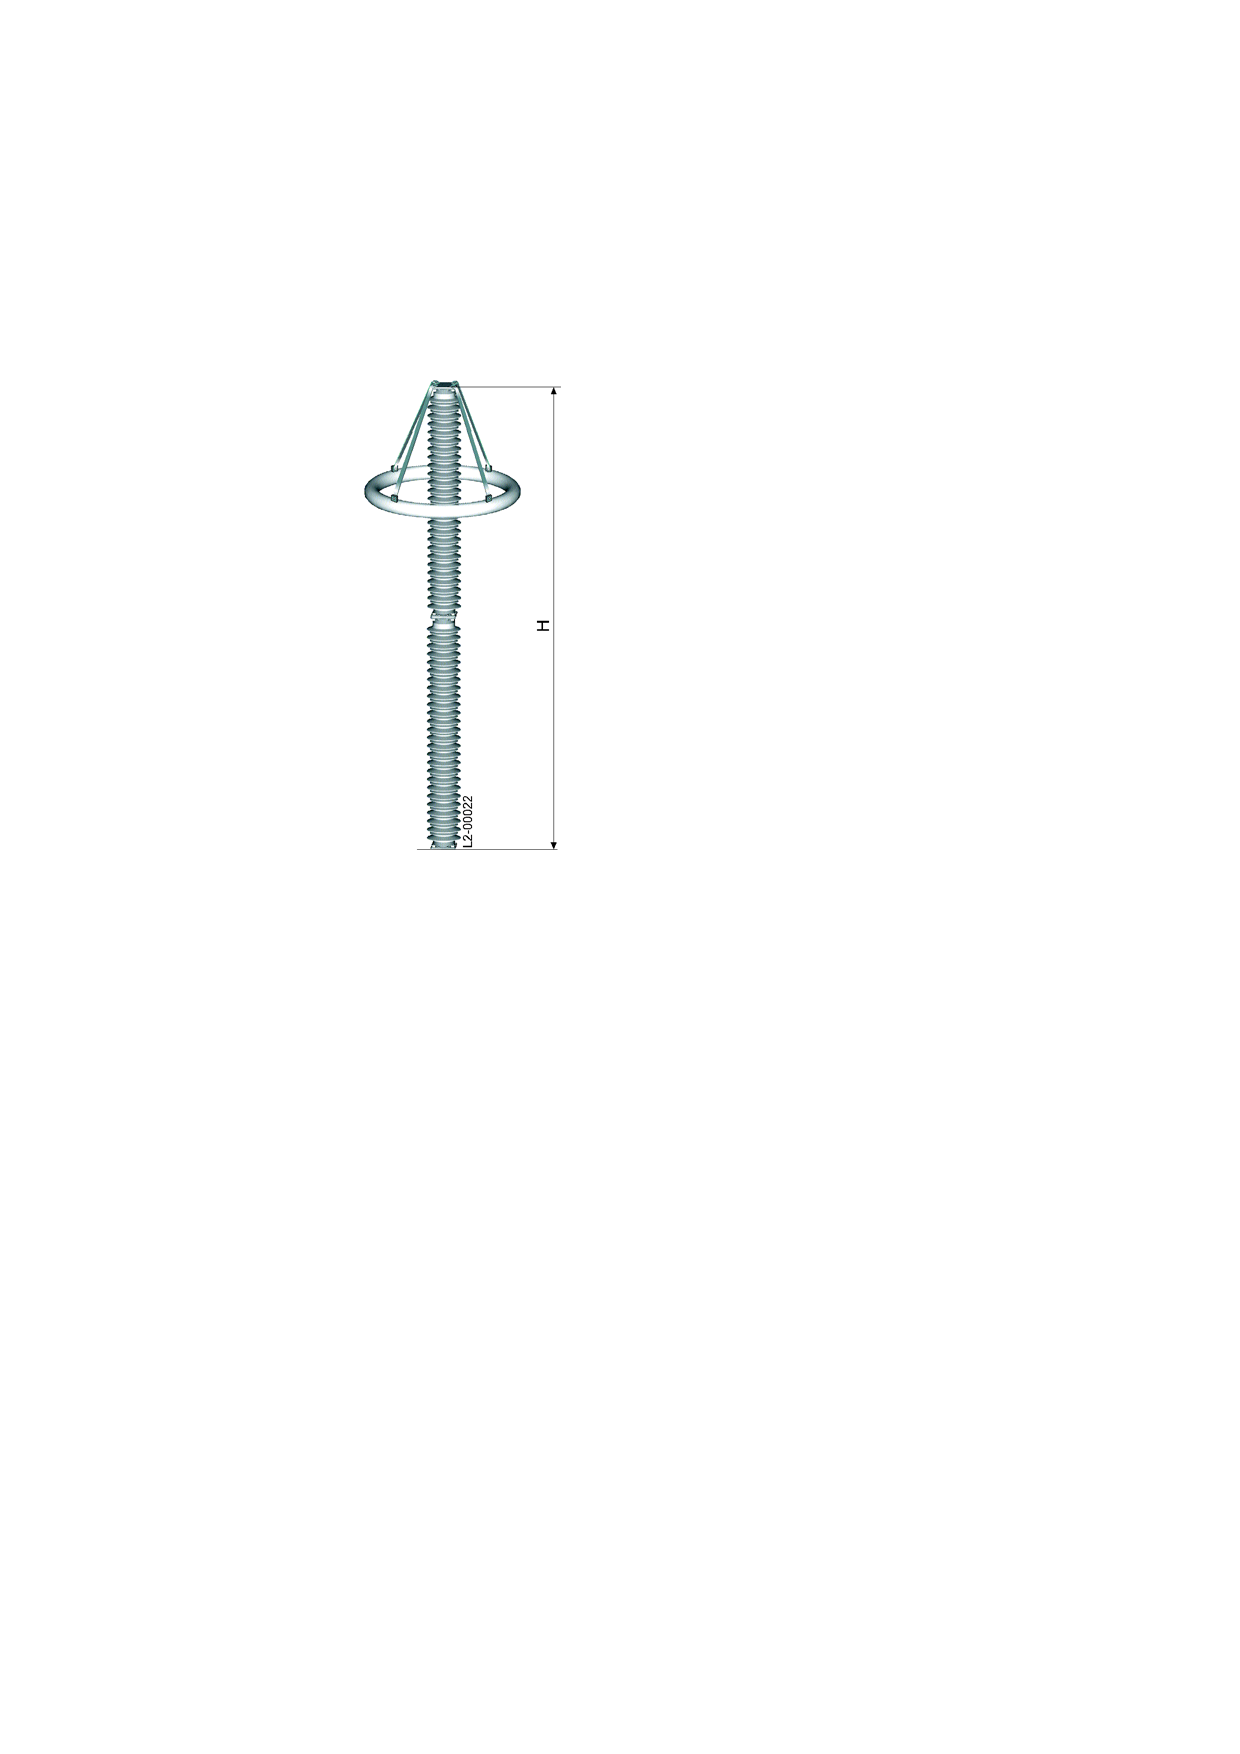
\includegraphics[width=2.7cm]{pararaio.pdf}
			\label{fig:pararaioA}
			}
			\subfloat[Placa de identificação] {
			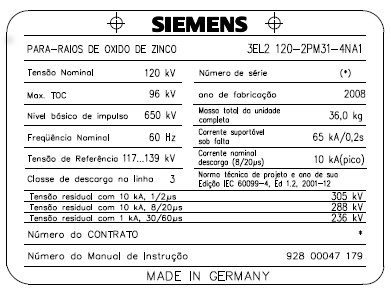
\includegraphics[width=8cm]{pararaio.jpg}
			\label{fig:pararaioB}
			}
			% \legend{Fonte: Do autor}
		\end{figure}

	\section{Muflas e Terminações}

	\section{Condutores}

	\section{Transformador de Corrente (TC)}
		Um transformador de corrente ou simplesmente TC é um dispositivo que reproduz no seu circuito secundário, a corrente que circula em um enrolamento primário com sua posição vetorial substancialmente mantida, em uma proporção definida, conhecida e adequada. Os transformadores de corrente, também chamados de transformadores de instrumentos, utilizados em aplicações de alta tensão (situações essas onde circulam, frequentemente, altas correntes), fornecem correntes suficientemente reduzidas e isoladas do circuito primário de forma a possibilitar o seu uso por equipamentos de medição, controle e proteção.\cite{mamedemanual}

		\subsection{Características construtivas}
			A seguir apresenta-se as diferentes formas para diferentes usos do TC.

			\subsubsection{Formas Construtivas}
				\paragraph*{a)\indent TC tipo barra}
					É aquele cujo enrolamento é constituído por uma barra fixada através do núcleo do transformador, conforme mostrado na \autoref{fig:tca}.
					\begin{figure}[htb]
						\caption{TC tipo barra}
						\centering
						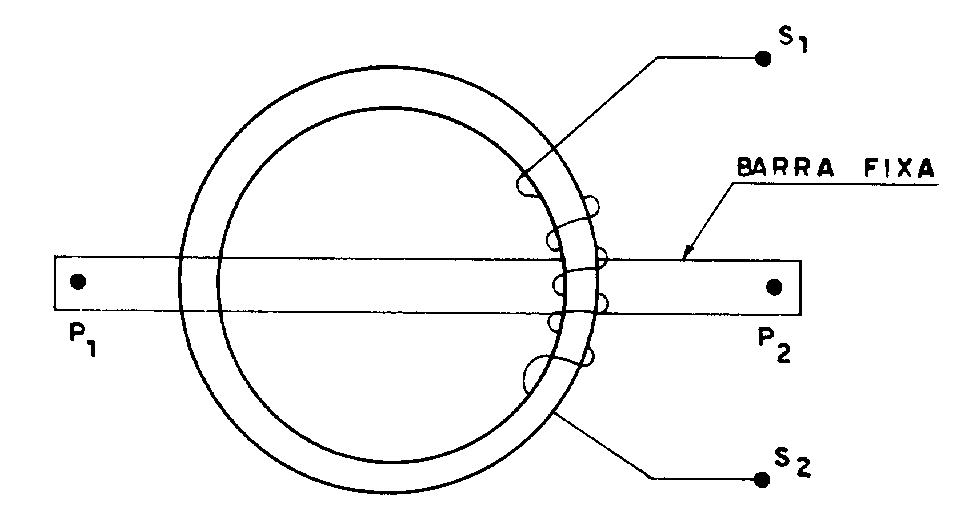
\includegraphics[width=5.4cm]{TC(1).png}
						% \legend{Fonte: Do autor}
						\label{fig:tca}
					\end{figure}
				\paragraph*{b)\indent TC tipo enrolado}
					É aquele cujo enrolamento é constituído de uma ou mais espiras envolvendo o núcleo do transformador, conforme ilustrado na \autoref{fig:tcb}.
					\begin{figure}[htb]
						\caption{TC tipo enrolado}
						\centering
						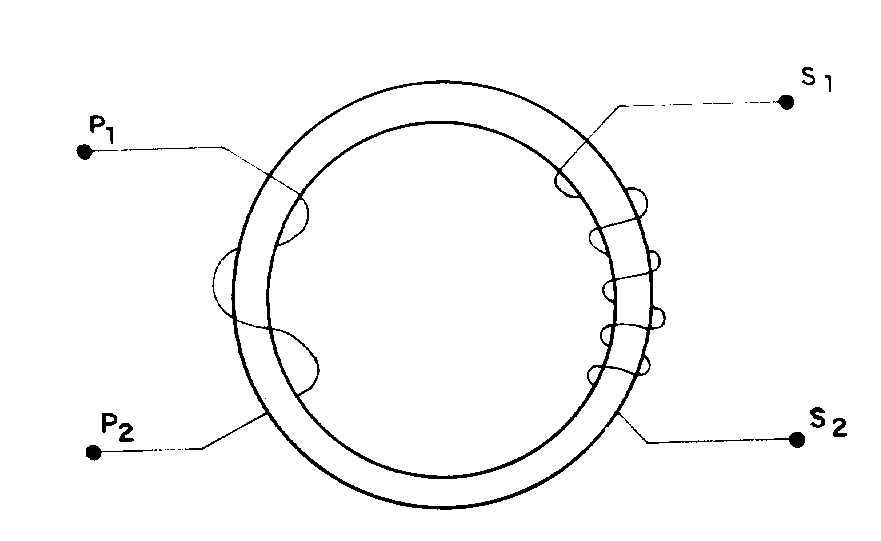
\includegraphics[width=5.4cm]{TC(2).png}
						% \legend{Fonte: Do autor}
						\label{fig:tcb}
					\end{figure}
				\paragraph*{c)\indent TC tipo janela}
					É aquele que não possui o primário fixo no transformador e é constituído de uma abertura através do núcleo, por onde passa o condutor que forma o circuito primário, conforme apresenta na \autoref{fig:tcc}.
					\begin{figure}[htb]
						\caption{TC tipo janela}
						\centering
						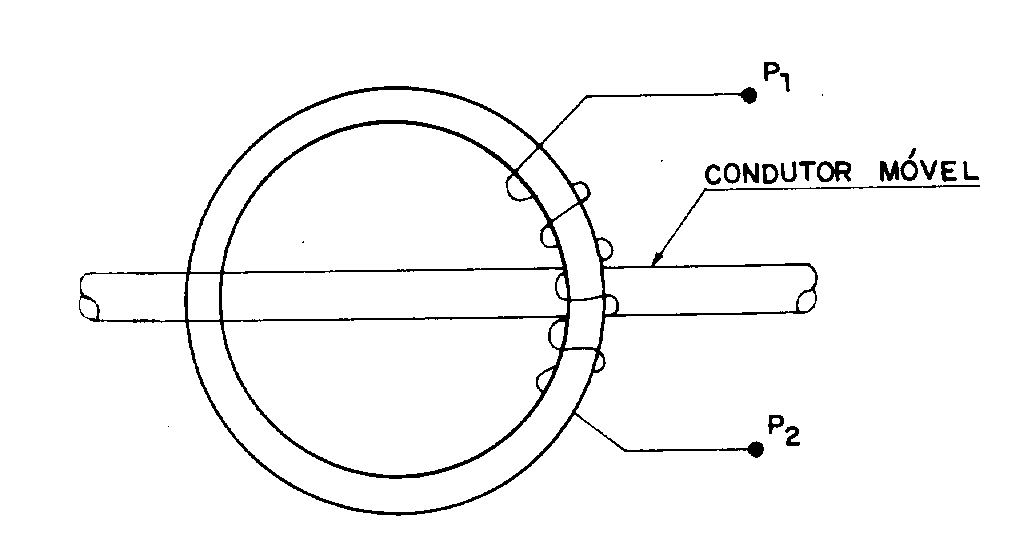
\includegraphics[width=5.4cm]{TC(3).png}
						% \legend{Fonte: Do autor}
						\label{fig:tcc}
					\end{figure}
				\paragraph*{d)\indent TC tipo bucha}
					É aquele cuja características são semelhantes às do tc do tipo barra, porém sua instalação é feita na bucha dos equipamentos, que funcionam como enrolamento primário, de acordo com a \autoref{fig:tcd}.
					\begin{figure}[htb]
						\caption{TC tipo bucha}
						\centering
						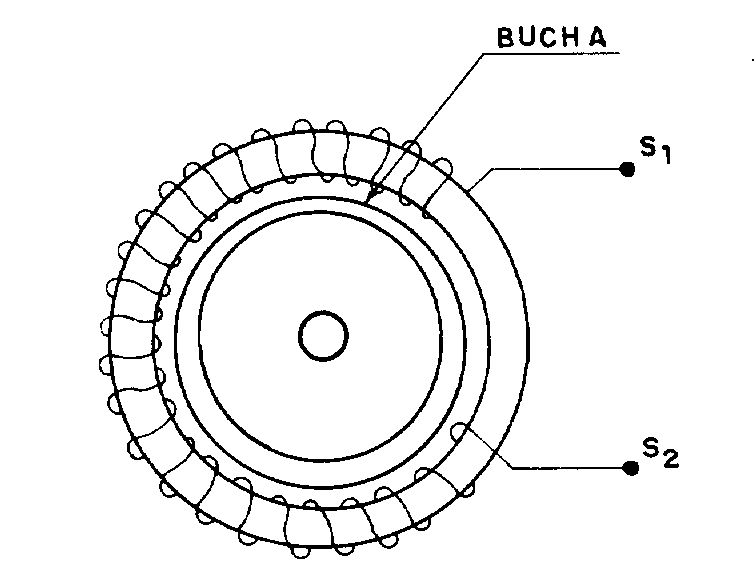
\includegraphics[width=5.4cm]{TC(4).png}
						% \legend{Fonte: Do autor}
						\label{fig:tcd}
					\end{figure}
				\paragraph*{e)\indent TC tipo núcleo dividido}
					É aquele cujas características são semelhantes às do tipo janela, em que o núcleo pode ser separado para permitir envolver o condutor que funciona como enrolamento primário, conforme se mostra na \autoref{fig:tce}.
					\begin{figure}[htb]
						\caption{TC tipo núcleo dividido}
						\centering
						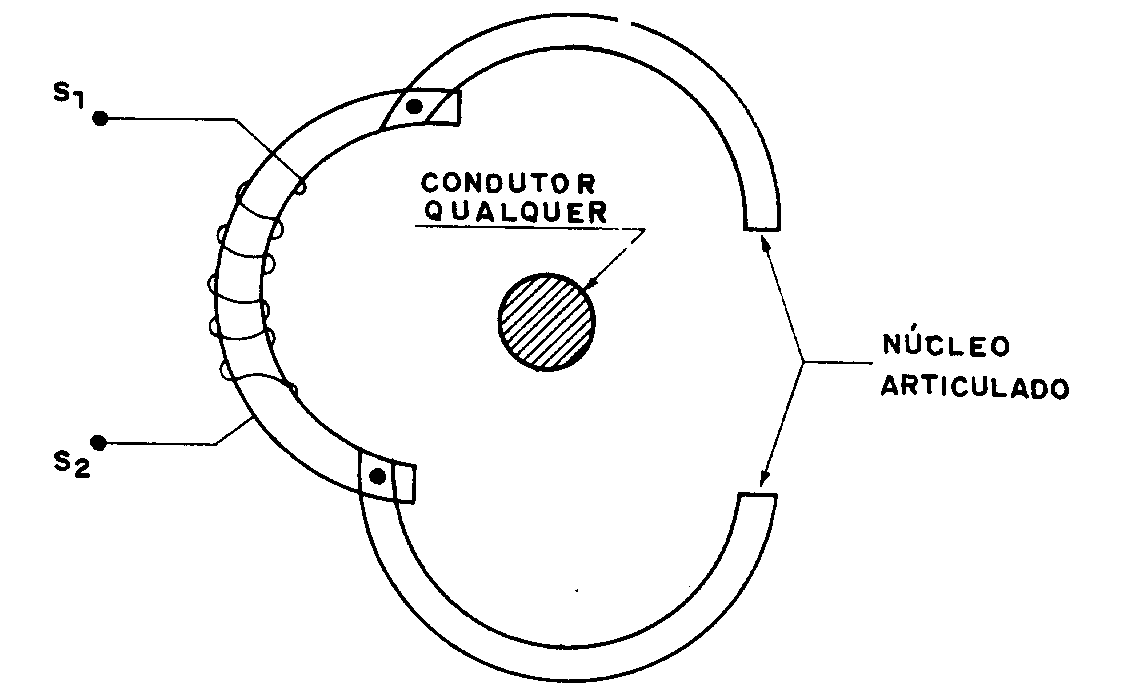
\includegraphics[width=5.4cm]{TC(5).png}
						% \legend{Fonte: Do autor}
						\label{fig:tce}
					\end{figure}
				\paragraph*{f)\indent TC tipo vários enrolamentos primários}
					É aquele constituído de vários enrolamentos primários montados isoladamente e apenas um enrolamento secundário, conforme a \autoref{fig:tcf}.
					\begin{figure}[htb]
						\caption{TC tipo vários enrolamentos primários}
						\centering
						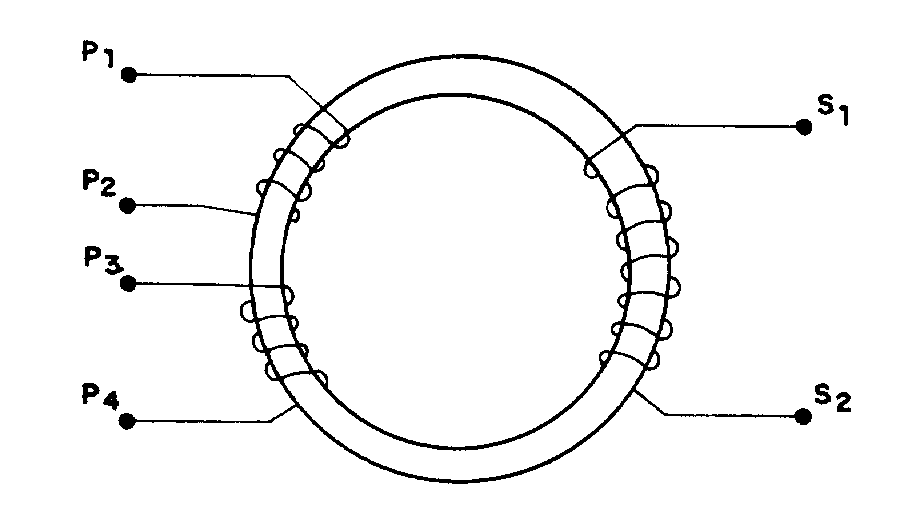
\includegraphics[width=5.4cm]{TC(6).png}
						% \legend{Fonte: Do autor}
						\label{fig:tcf}
					\end{figure}
				\paragraph*{g)\indent TC tipo vários núcleos secundários}
					É aquele constituído de dois o mais núcleos secundários montados isoladamente formando com o enrolamento primário, um só conjunto, conforme se mostra na \autoref{fig:tcg}.
					\begin{figure}[htb]
						\caption{TC tipo vários núcleos secundários}
						\centering
						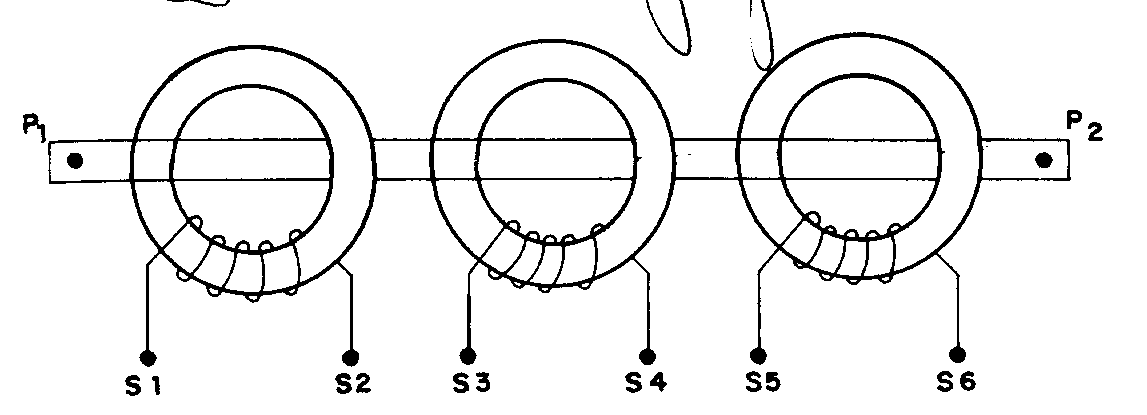
\includegraphics[width=5.4cm]{TC(7).png}
						% \legend{Fonte: Do autor}
						\label{fig:tcg}
					\end{figure}
				\paragraph*{h)\indent TC tipo vários enrolamentos secundários}
					É aquele constituído de um núcleo envolvido pelo enrolamento primário e vários enrolamentos secundários, conforme se mostra na \autoref{fig:tch}, e que podem ser ligados em série ou paralelo.
					\begin{figure}[htb]
						\caption{TC tipo vários enrolamentos secundários}
						\centering
						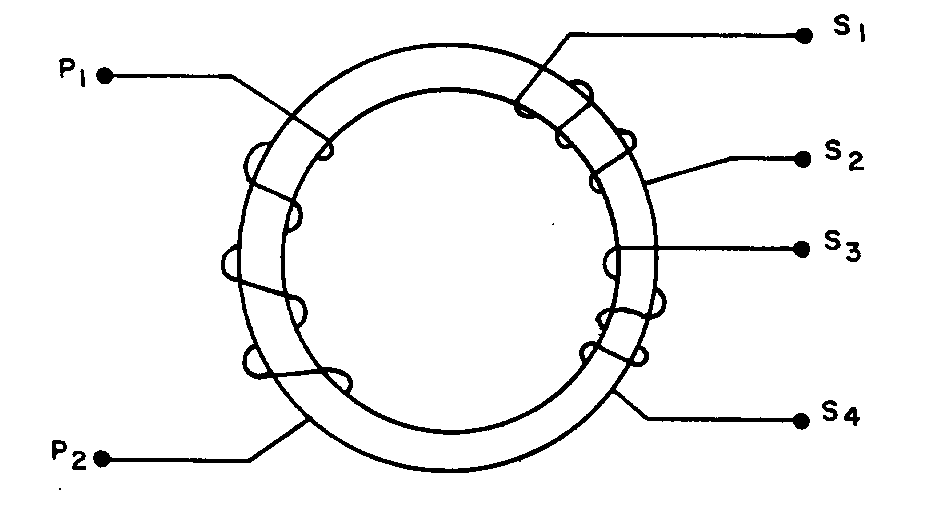
\includegraphics[width=5.4cm]{TC(8).png}
						% \legend{Fonte: Do autor}
						\label{fig:tch}
					\end{figure}
				\paragraph*{i)\indent TC tipo derivação no secundário}
					É aquele constituído de um único núcleo envolvido pelo enrolamentos primário e secundário, sendo este promovido de uma ou mais derivações. Entretanto, o primário pode ser constituído de um ou mais enrolamentos, conforme se mostra na \autoref{fig:tcf}. Como os ampères-espiras variam em cada relação de transformadores considerada, somente é garantida a classe de  exatidão do equipamento para a derivação que contiver o maior número de espiras. A versão desse tipo de TC é apresentado na \autoref{fig:tci}.  
					\begin{figure}[htb]
						\caption{TC tipo derivação no secundário}
						\centering
						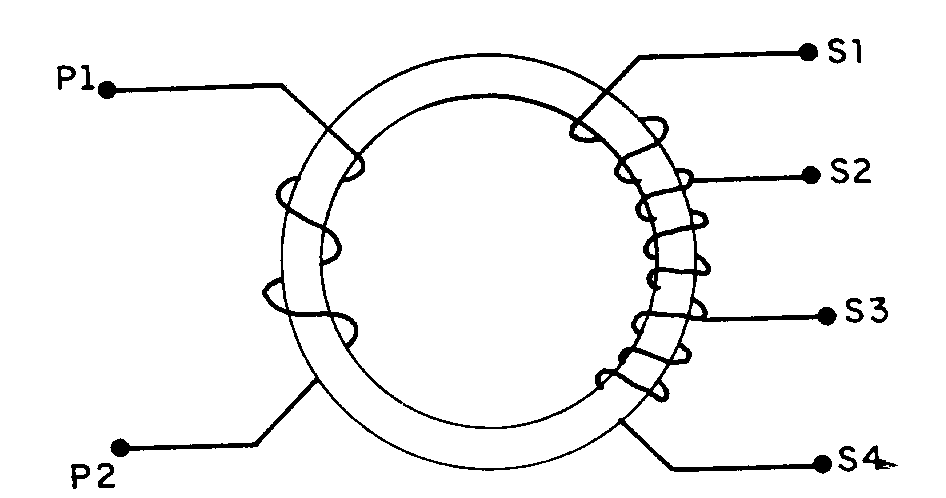
\includegraphics[width=5.4cm]{TC(9).png}
						% \legend{Fonte: Do autor}
						\label{fig:tci}
					\end{figure}
				\paragraph*{j)\indent TC de barra do tipo relação múltiplas com primário em várias seções}
					É aquele constituído de múltiplas barras no primário que podem ser ligadas em série-paralelo formando múltiplas relações.
			
			\subsubsection{Tipos de isolamento}
				\paragraph*{a)\indent TCs de baixa tensão}
					Os núcleo e os enrolamentos são encapsulados em resina epóxi que os torna rígidos, tornando-os compactos com características eletromecânicas de grande desempenho. Porém o epóxi tem a desvantagem de ser descartável depois de uma falha interna não sendo possível sua recuperação.
				\paragraph*{b)\indent TCs de média e alta tensão}
					Para a média tensão o isolamento pode ser em resinas sintéticas e a óleo mineral isolante, geralmente imerso num tanque metálico cheio de óleo. Agora os terminais constituídos por isoladores de porcelana.\par
					Para a alta tensão é usado porcelana-óleo e a hexafluoreto de enxofre ($SF_6$).\par

		\subsection{Características Elétricas}
			O circuito equivalente padrão dos transformadores de corrente mostra os terminais primários de alta tensão P1 e P2 e os terminais secundários S1 e S2, como visto na \autoref{fig:tc2}.\par
			\begin{figure}[htb]
				\caption{Simbologia e circuito equivalente simplificado do TC}
				\centering
				\subfloat [Simbologia]{
				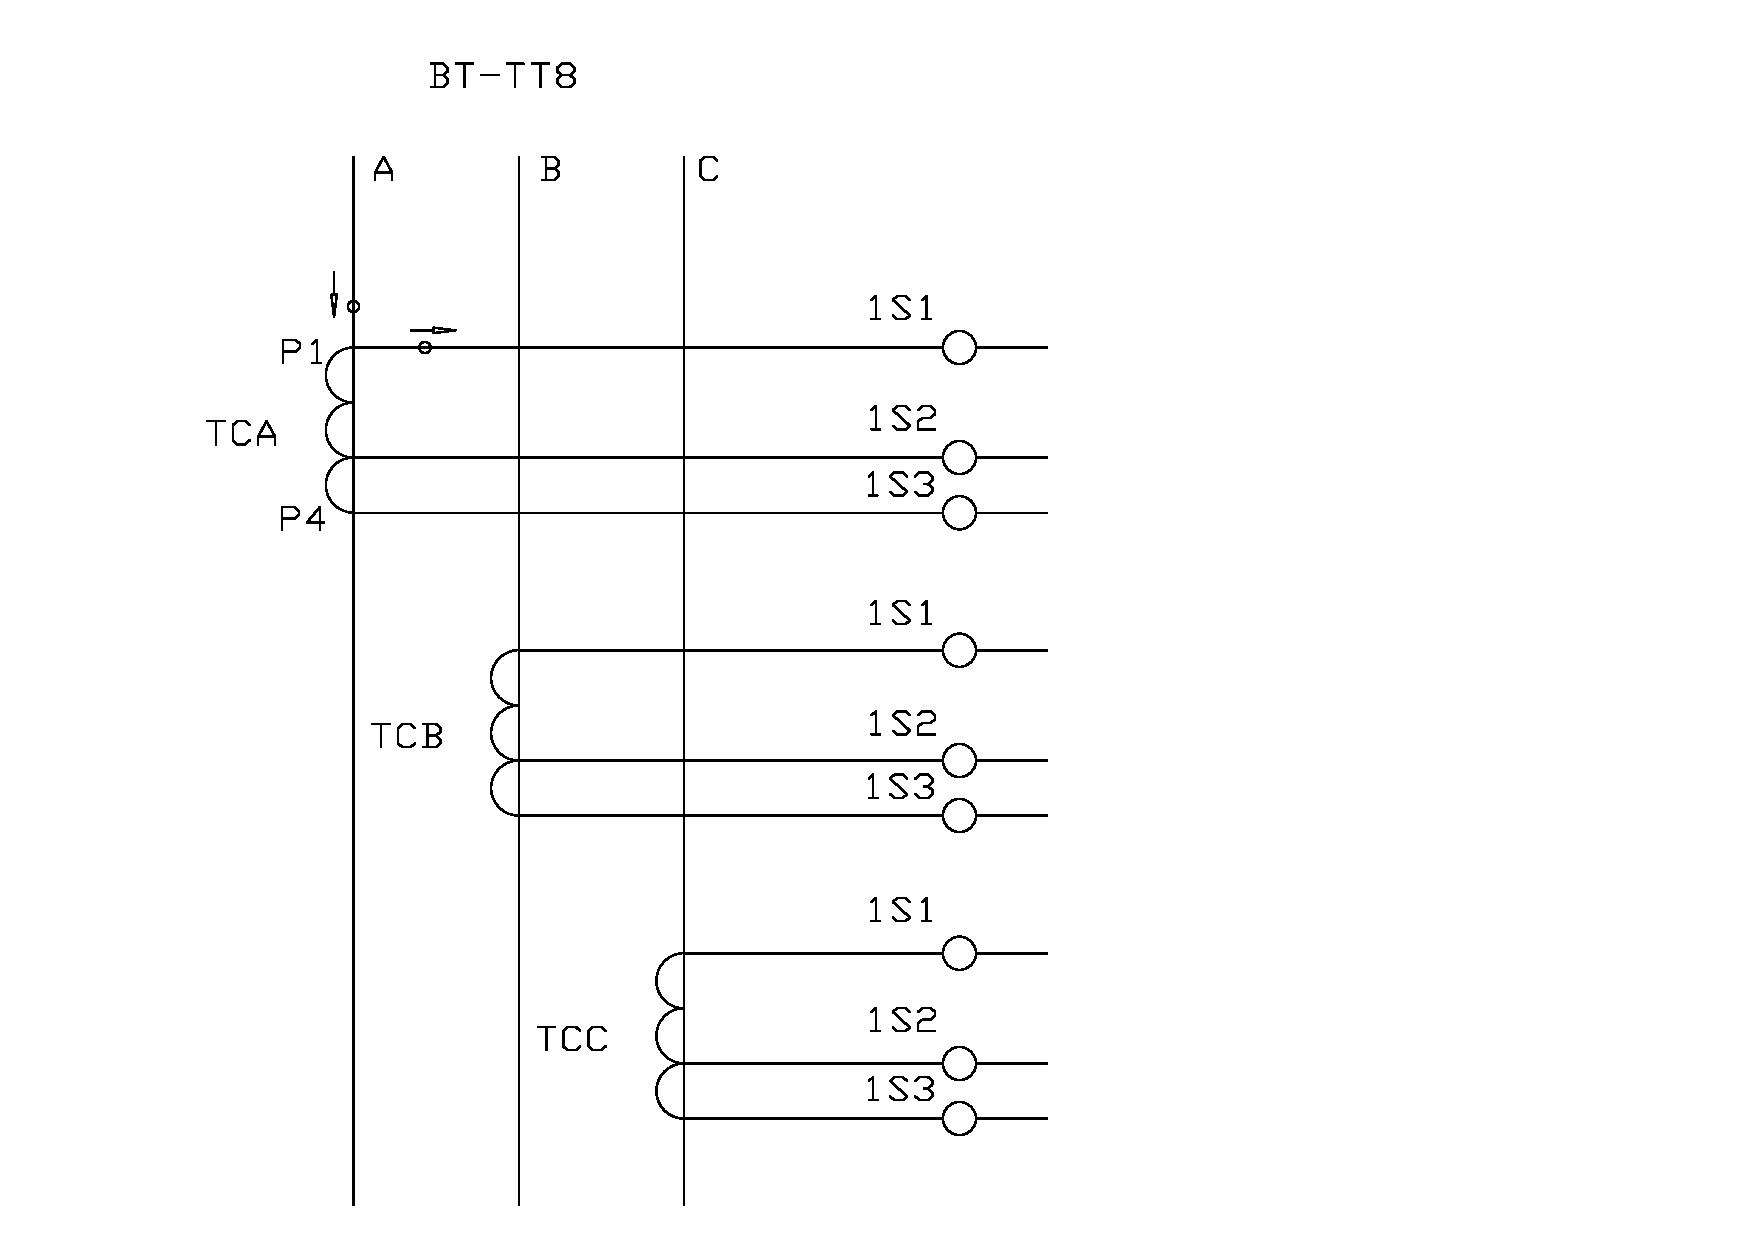
\includegraphics[width=5cm]{tca.pdf}
				\label{fig:tc1}
				}
				\subfloat [Circuito equivalente]{
				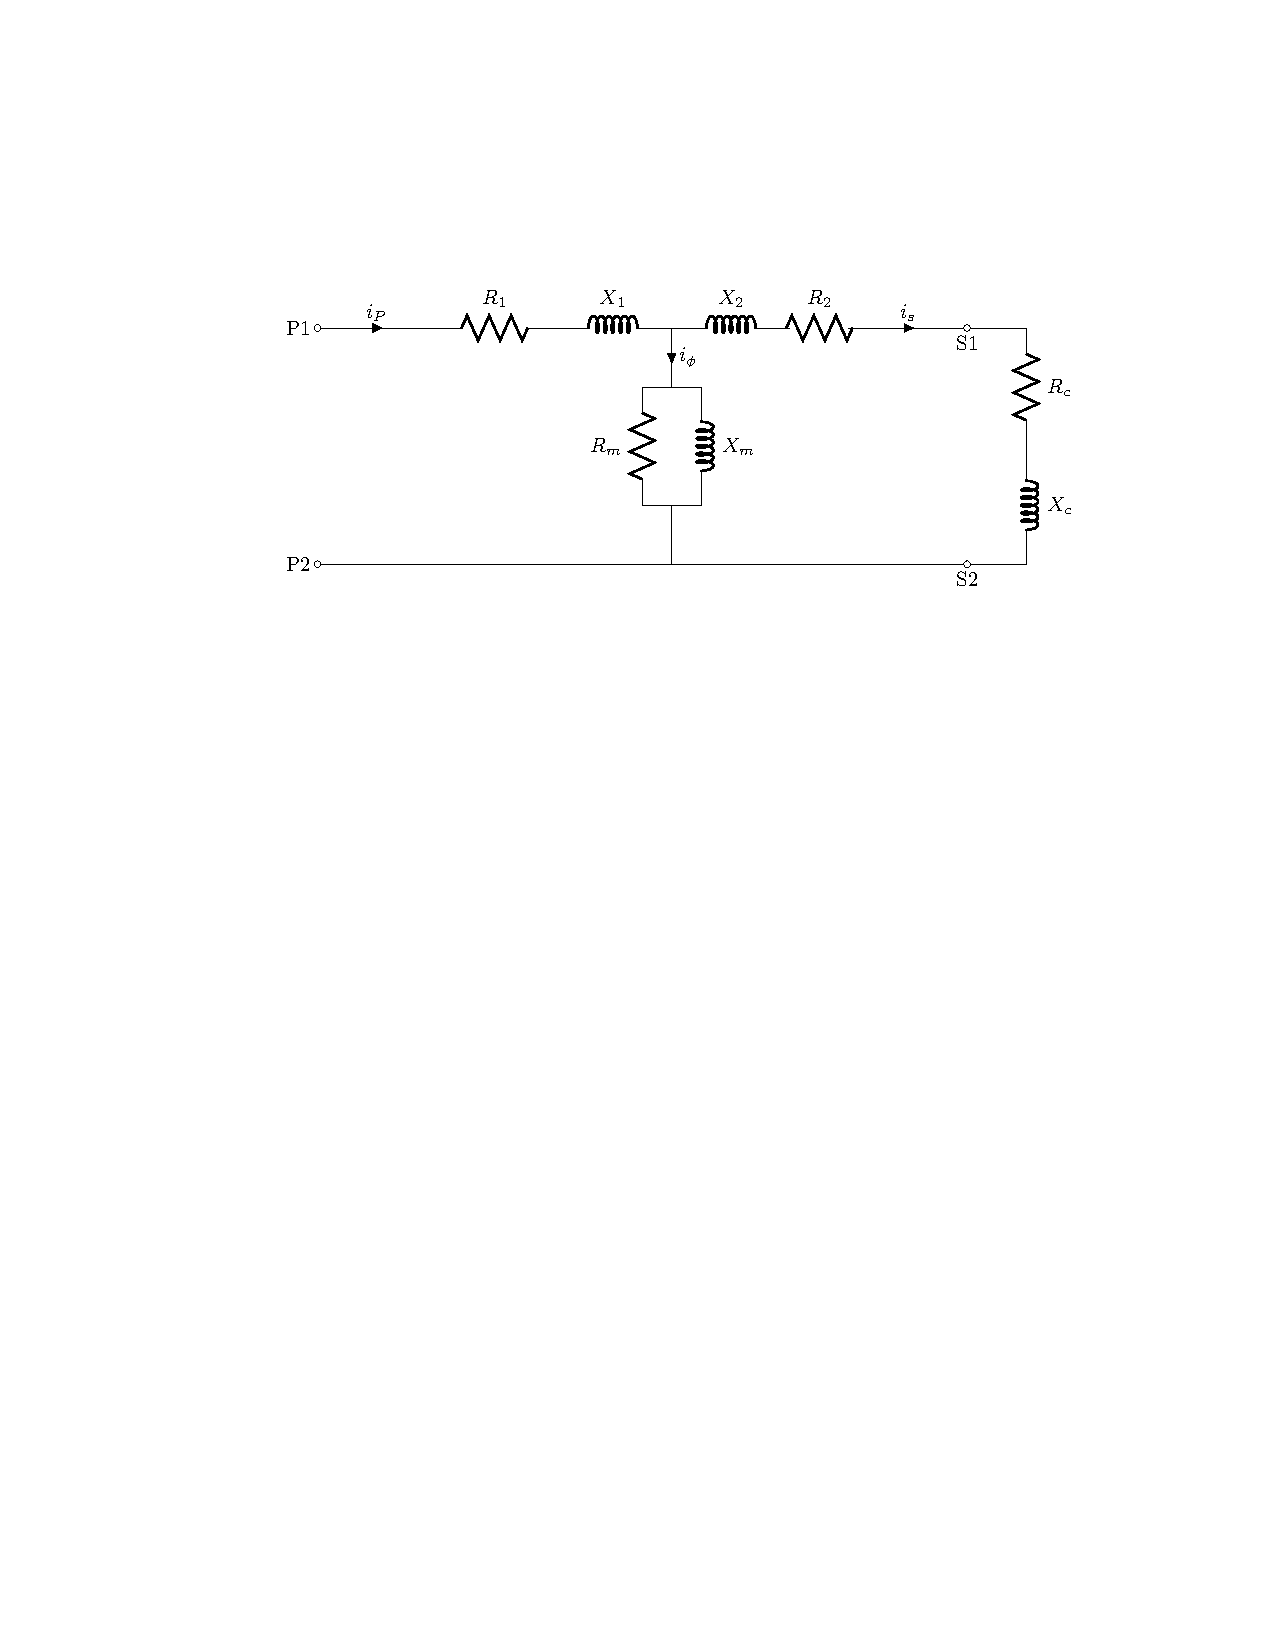
\includegraphics[width=5.8cm]{tcb.pdf}
				\label{fig:tc2}
				}
				\legend{Fonte: Do autor}
				\end{figure}
			
			O ponto para transformadores com polaridade aditiva, mostrado na \autoref{fig:tc1} indica onde entra a corrente no primário e onde sai a corrente no secundário (defasagem de 180º). Modelos industriais de TC’s têm os terminais de alta tensão marcados como P1 e P2 (Primário 1 e Primário 2), sendo que em muitos casos pode haver diferentes ligações do circuito primário com diferente relação de transformação. Os terminais secundários são marcados como 1S1, 1S2, 1S3, indicando respectivamente o número do enrolamento, o símbolo de terminal secundário (s) e o número da derivação do terminal secundário. Na \autoref{fig:tc1} é mostrado a simbologia de três TC's nas fases A, B e C da baixa tensão de um transformador.\par
			O circuito equivalente, de modo geral, para um transformador de corrente pode ser modelado como no esquema da \autoref{fig:tc2}. Onde as resistências e as reatâncias com índice 1 são relativas ao primário, as com índice 2 são relativas ao secundário e o núcleo de ferro do acoplamento magnético representado com o índice m onde o $R_m$ representa as perdas ôhmicas através das correntes de histerese e de Foulcault e $X_m$ responsável pela corrente reativa devida à circulação das linhas de fluxo do circuitos magnético. \cite{mamedemanual}\par
			Pela \autoref{fig:tc2} pode-se entender que a uma corrente $I_p$ absorvida da rede provoca uma queda de tensão no primário, em seguida é transmitida ao secundário que alimenta a bobina secundária e a bobina do galvanômetro (ou medidor digital) representado pela impedância $Z_c=R_c+iX_c$. As perdas do núcleo por meio da corrente $I_\phi$ determinam o erro de medição, com isto é possível calcular a corrente do secundário por $I_s=I_p-I_\phi$.\par
			\begin{figure}[htb]
				\caption{Foto de um Transformador de Corrente}
				\centering
				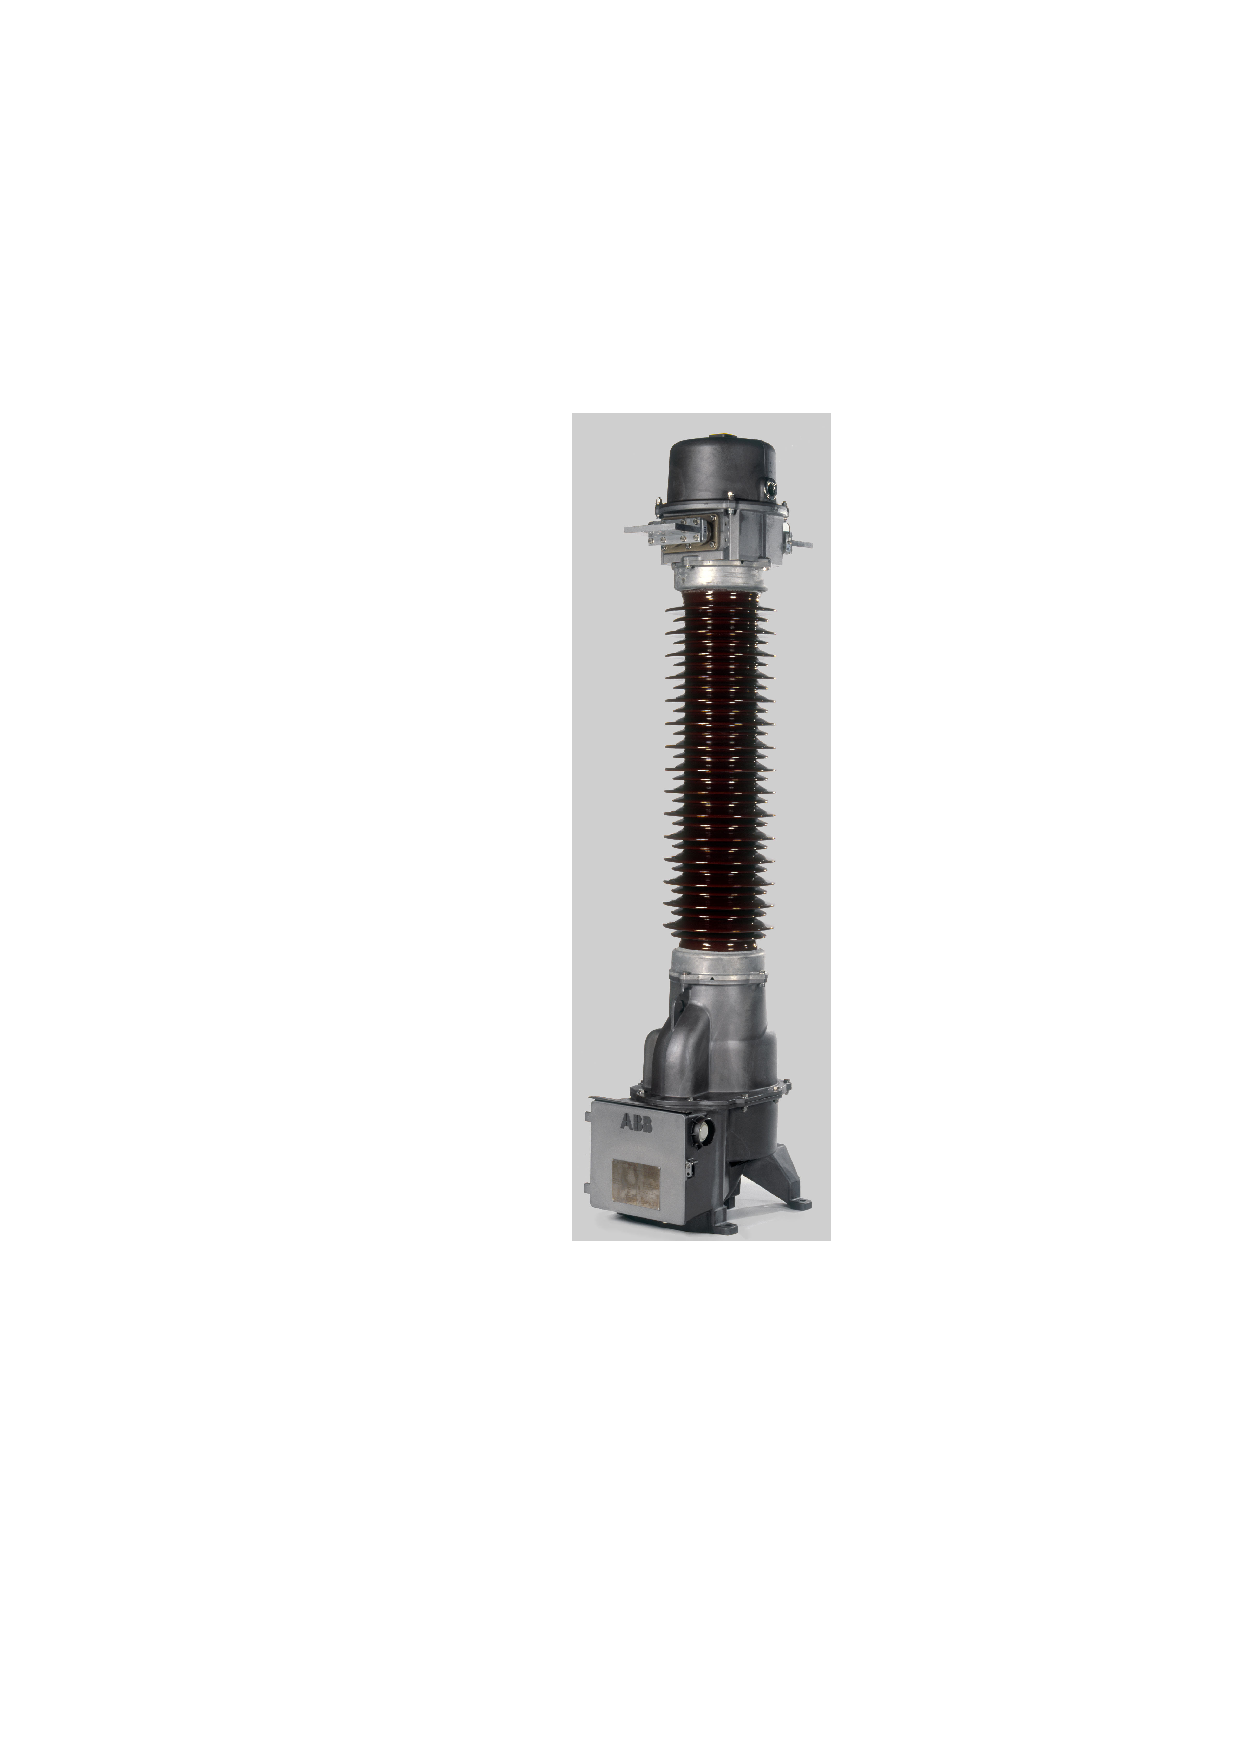
\includegraphics[width=3cm]{fototc.pdf}
				\legend{Fonte: Do autor}
				\label{fig:fototc}
				\end{figure}
			\subsubsection{Correntes Nominais}
			\subsubsection{Cargas Nominais}			
			\subsubsection{Fator de Sobrecorrente}
			\subsubsection{Corrente de Magnetizaçao}
			\subsubsection{Tensão Secundária}
			\subsubsection{Fator Térmico Nominal}
			\subsubsection{Corrente Térmica Nominal}
			\subsubsection{Fator Térmico de Curto-circuito}
			\subsubsection{Corrente Dinâmica Nominal}
			\subsubsection{Tensão Suportável à Frequência Industrial}
			\subsubsection{Polaridade}



		\subsection{Classificação}
			\subsubsection{TCs para serviço de medição}
				São os transforadores cuja função é medir, requer reproduzir fielmente a magnitude e o ângulo de fase da corrente, sua precisão deve ser garantida desde uma pequena fração de corrente nominal da ordem de 10\% até o excesso de corrente da ordem de 20\%, sobre o valor nominal.\cite{apuntesmeza}\par
			\subsubsubsection{Fator de sobrecorrente}
				Além de representar uma elevada segurança aos operadores e leituristas, os TCs têm a finalidade de proteger os instrumentos de medida contra sobrecargas ou sobrecorrentes de valores muito elevados. Isto é possível, porque o seu núcleo é especificado para entrar em saturação para correntes superiores à corrente nominal vezes o fator de sobrecorrente, conforme se pode mostrar na \autoref{eq:fsobrecorrente}.
				\begin{equation} \label{eq:fsobrecorrente}
					F_{s} = \frac{I_{ps}}{I_{np}}
					\end{equation}

			\subsubsection{TCs para serviço de proteção}
				São os transformadores cuja função é proteger um circuito, requer conservar sua fidelidade até um valor de vinte vezes a magnitude de corrente nominal, quando trata-se de grande redes com altas correntes poder ser necessário requerer trinta vezes a corrente nominal.\par
				No caso dos relés de sobrecorrente, só importa a relação de transformação, mas em outros tipos de relés, como pode ser os de impedância, é requerido além da relação de transformação, manter o erro do ângulo de fase dentro dos valores predeterminados.\cite{apuntesmeza}\par

	\section{Transformador de Potencial (TP)}

	\section{Chave seccionadora}

	\section{Painéis}

	\section{Disjuntor}

	\section{Transformador de Potência}

	\section{Capacitores de Potência}

	\section{Resistores de Aterramento}

	\section{Reguladores de Tensão}

	\section{Religadores Automáticos}

	\section{Relés}


% ---------------------------------------------------
% Capítulo 2
% ---------------------------------------------------

\chapter{Projeto de subestações de alta tensão}
	\label{chap:projSEAT}
	A \citeonline{IEC60038:2002} define os circuitos de alta tensão como sendo aqueles com tensões acima de 1000V em corrente alternada. No presente capítulo serão abordados os diferentes tipos de configuração de barra de subestações de distribuição, ou seja, entre 13,8kV e 138kV. Far-se-á primeiramente algumas definições. 

	\section{Introdução}
		Segundo \citeonline{book:equipAT} o módulo de manobra consiste no conjunto de equipamentos, materiais e serviços necessários à implantação dos setores de manobra. Todavia outra denominação usualmente usada como vãos, ou na sua denominação em inglês \textit{bay}, em seu cerne, estas denominações caracterizam o espaço físico para realização de funções (manobras) que permitem a composição da subestação em módulos. Ao longo do capítulo, ficará claro que a subestação pode ser montada como uma espécie de LEGO, cujos diversos tipos de \textit{bays} podem se encaixar conforme necessidade e espaço físico disponível. Os principais vãos (ou módulos de manobra, ou \textit{bays}) em subestações podem ser definidas como:\par

		\begin{itemize}
			\item Entrada de Linha (EL)
			\item Interligação de Barramentos (IB)
			\item Conexão de Auto/Transformador (CT)
			\item Alimentador (AL)
			\end{itemize}
		\subsection{Entrada de Linha (EL)}
			A entrada de linha consiste na fonte de energia que alimenta a subestação. Os padrões provém segundo a \citeonline{nt304}.\footnote{A NT409 informa sobre a metodologia de composição dos módulos construtivos do sistema brasileiro de distribuição de energia elétrica, referente às redes, linhas e subestações de distribuição, com tensão inferior a 230 kv. metodologia de composição dos módulos construtivos do sistema brasileiro de distribuição de energia elétrica, referente às redes, linhas e subestações de distribuição, com tensão inferior a 230 kv}\par
			A \autoref{fig:ELcorte} mostra o arranjo padrão para entradas de linha em 138kV, verifica-se a utilização do para-raio (PR) como primeiro equipamento para proteção dos equipamentos subsequentes contra descargas atmosféricas, equipamentos de proteção como os transformadores de potencial (TP) e corrente (TC), derivação para as chaves seccionadoras que se dirigem para o disjuntor (DJ) principal (seccionadoras normalmente fechadas) e para o disjuntor TIE (seccionadoras normalmente abertos, caso os disjuntor principal não esteja em manutenção), e a presença dos dois barramentos para execução da manobra de manutenção dos disjuntores.\par
			\begin{figure}[!b]
				\caption{Corte Lateral de uma Entrada de Linha}
				\centering
				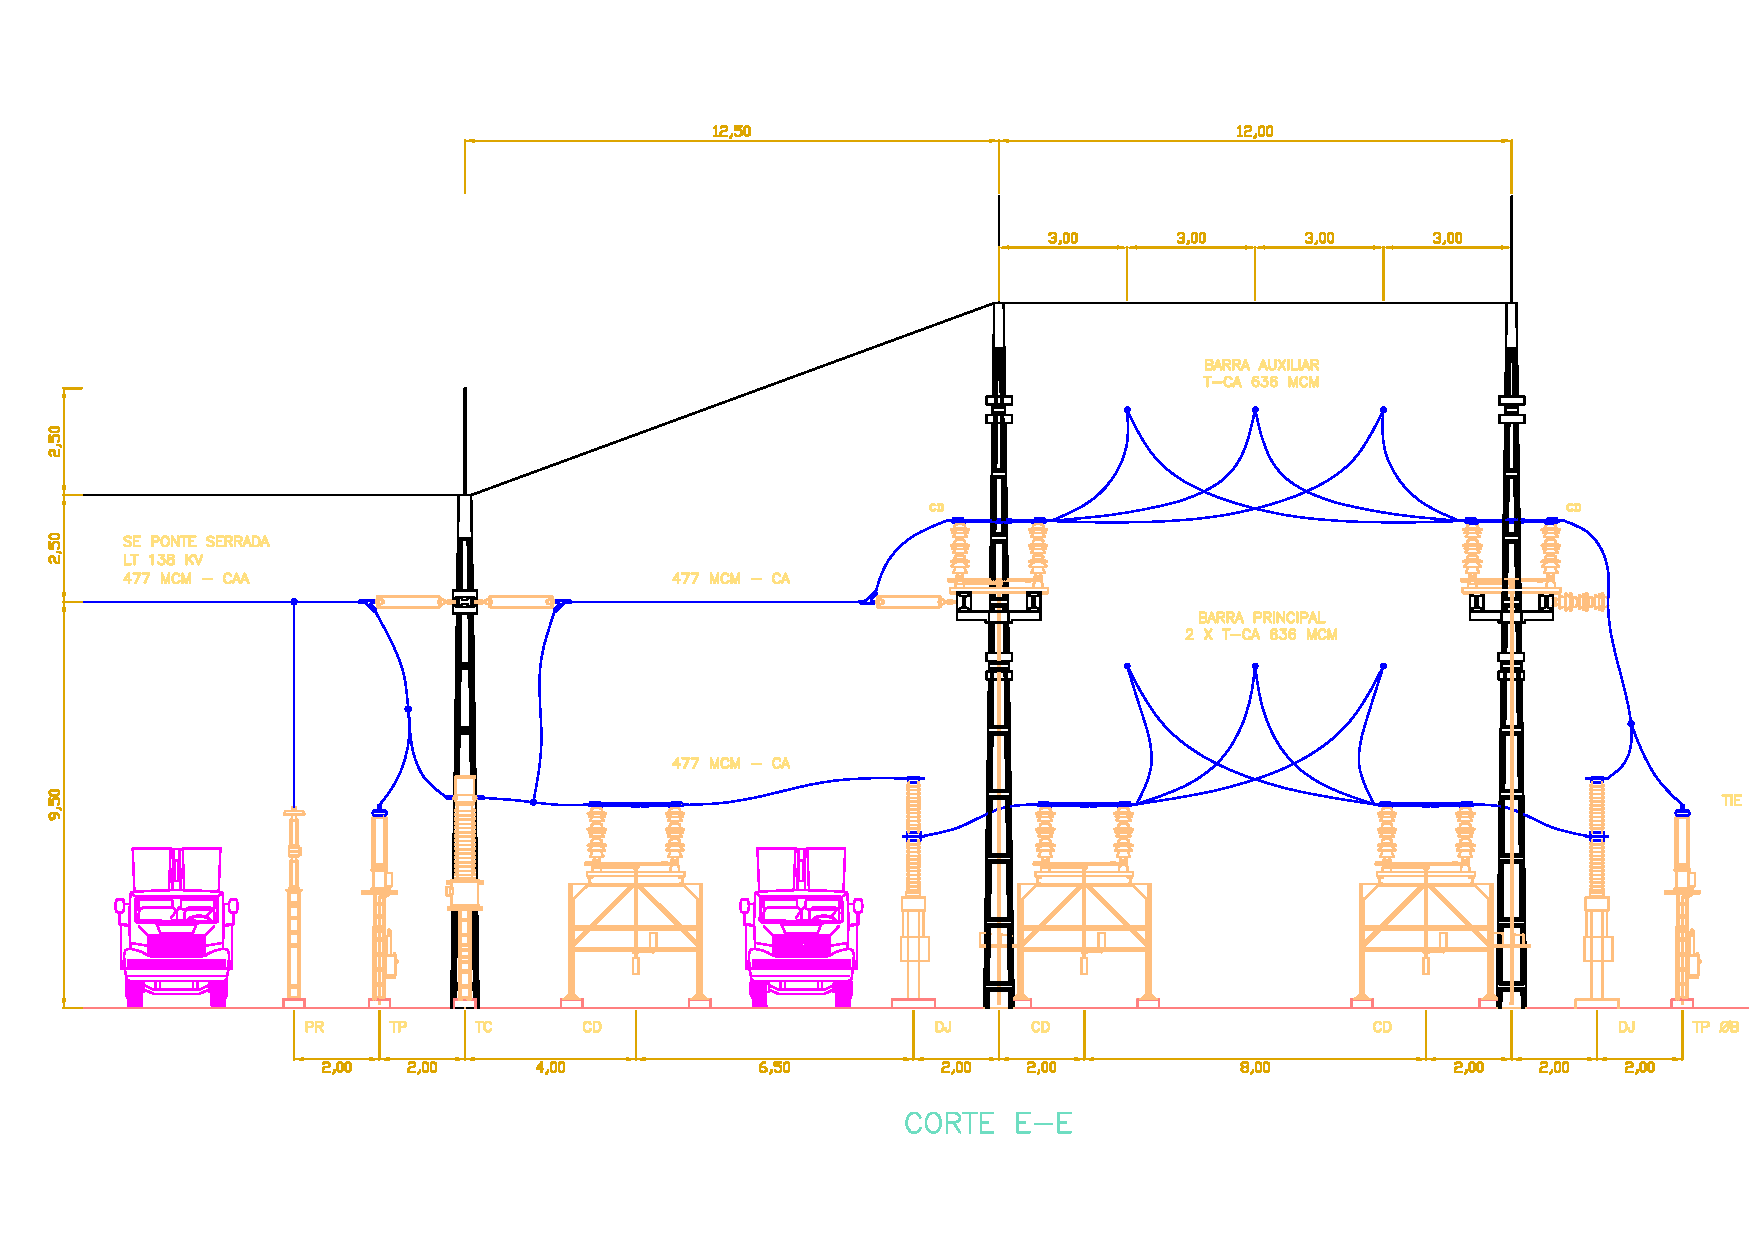
\includegraphics[width=150mm,angle=90]{ELcorte.pdf}
				\legend{Fonte: Cedido por Celesc S.A. - Subestação Concórdia São Cristóvão - 138/34/13,8kV}
				\label{fig:ELcorte}
				\end{figure}
		\subsection{Conexão de Auto/Transformador (CT)}
			A conexão de transformador liga o barramento ao transformador. A \autoref{fig:UNCT} mostra no lado de alta a conexão em barra principal e de transferência com proteção do disjuntor ligado na barra principal, derivação com uma chave para a barra de transferência. No lado de baixa, a conexão é feita em barra simples comum nestes níveis de tensão, onde se utiliza apenas um \textit{baypass} com uma chave seccionadora.\par
			Já a \autoref{fig:CTcorte} mostra um exemplo de conexão de transformador quando a alta é ligado aos dois barramentos.\par
			\begin{figure}[!b]
				\caption{Diagrama unifilar de uma conexão de transformador}
				\centering
				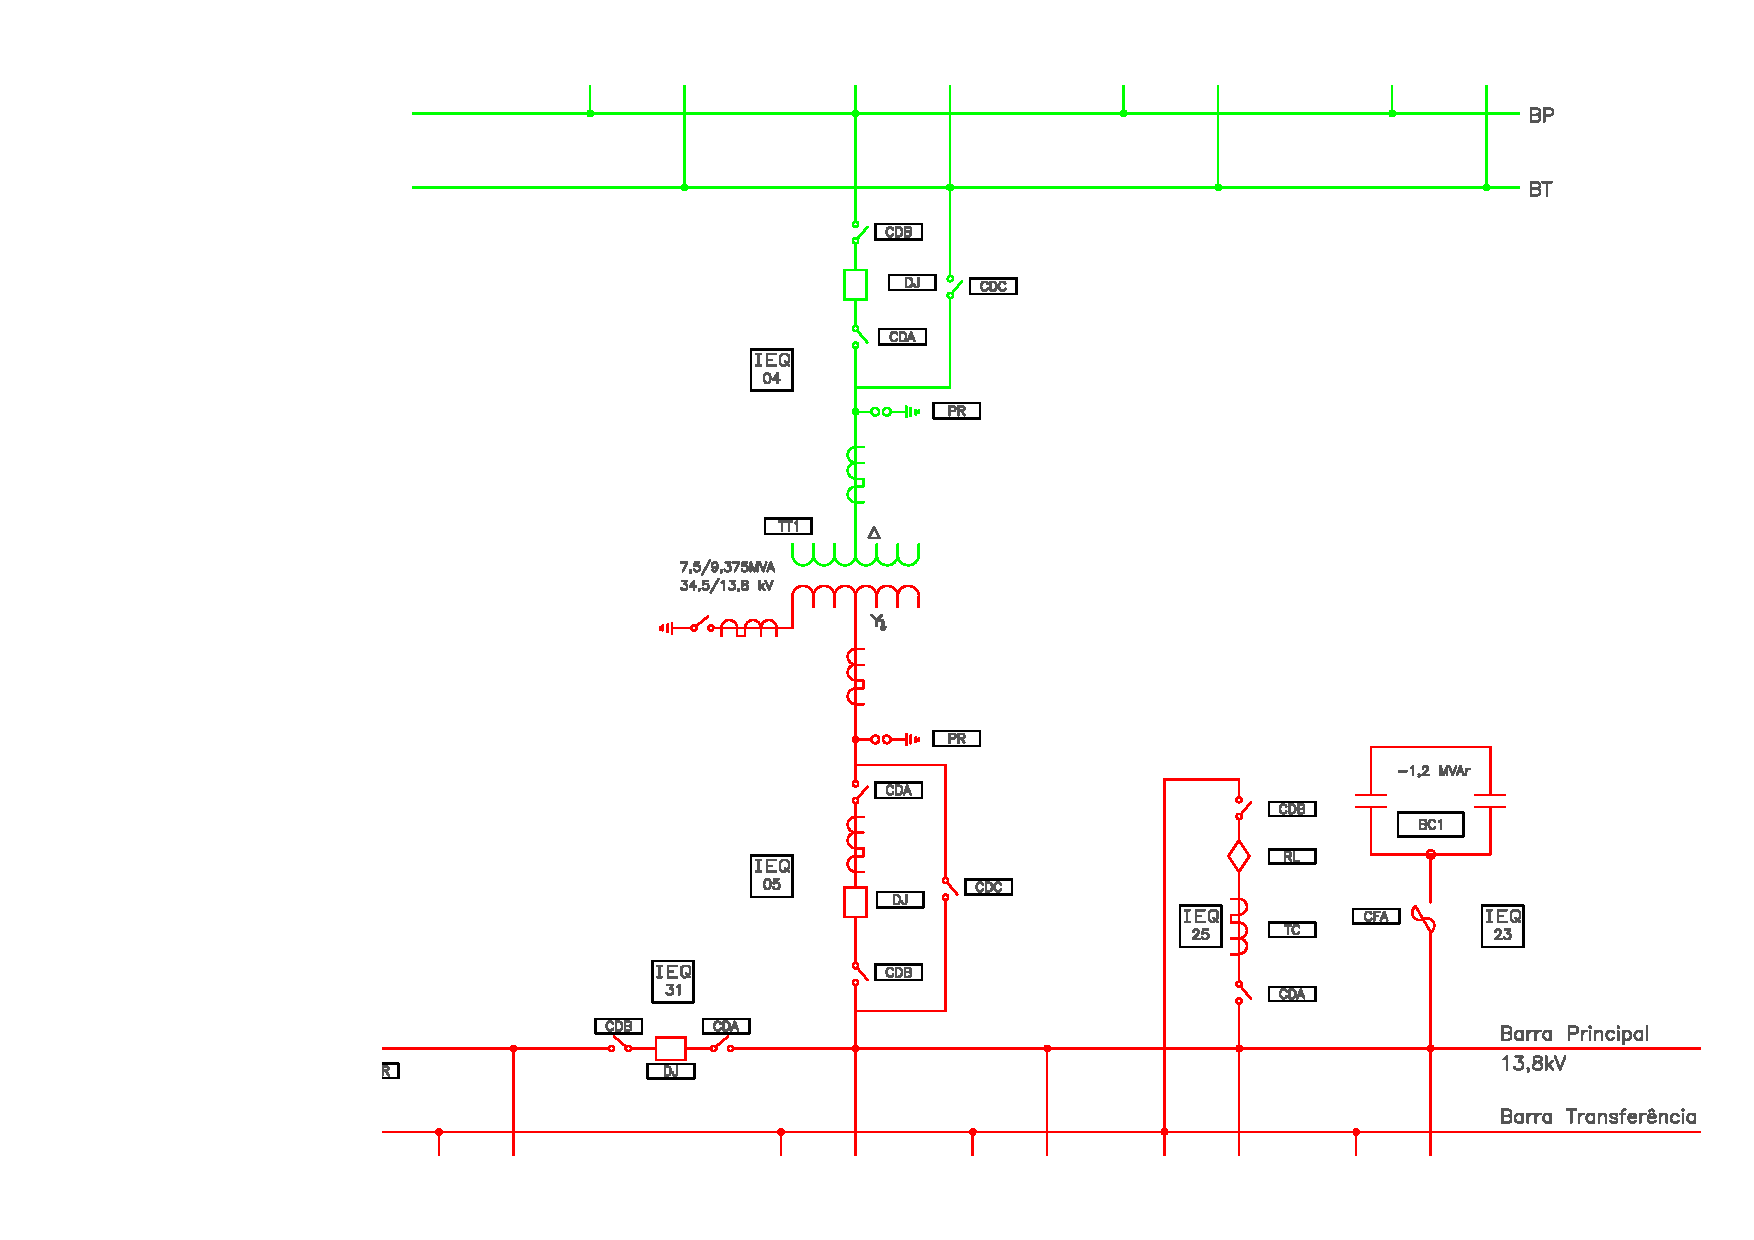
\includegraphics[width=108mm]{UNCT.pdf}
				\legend{Fonte: Do autor}
				\label{fig:UNCT}
				\end{figure}
			\begin{figure}[!b]
				\caption{Corte de uma conexão de transformador em 138kV}
				\centering
				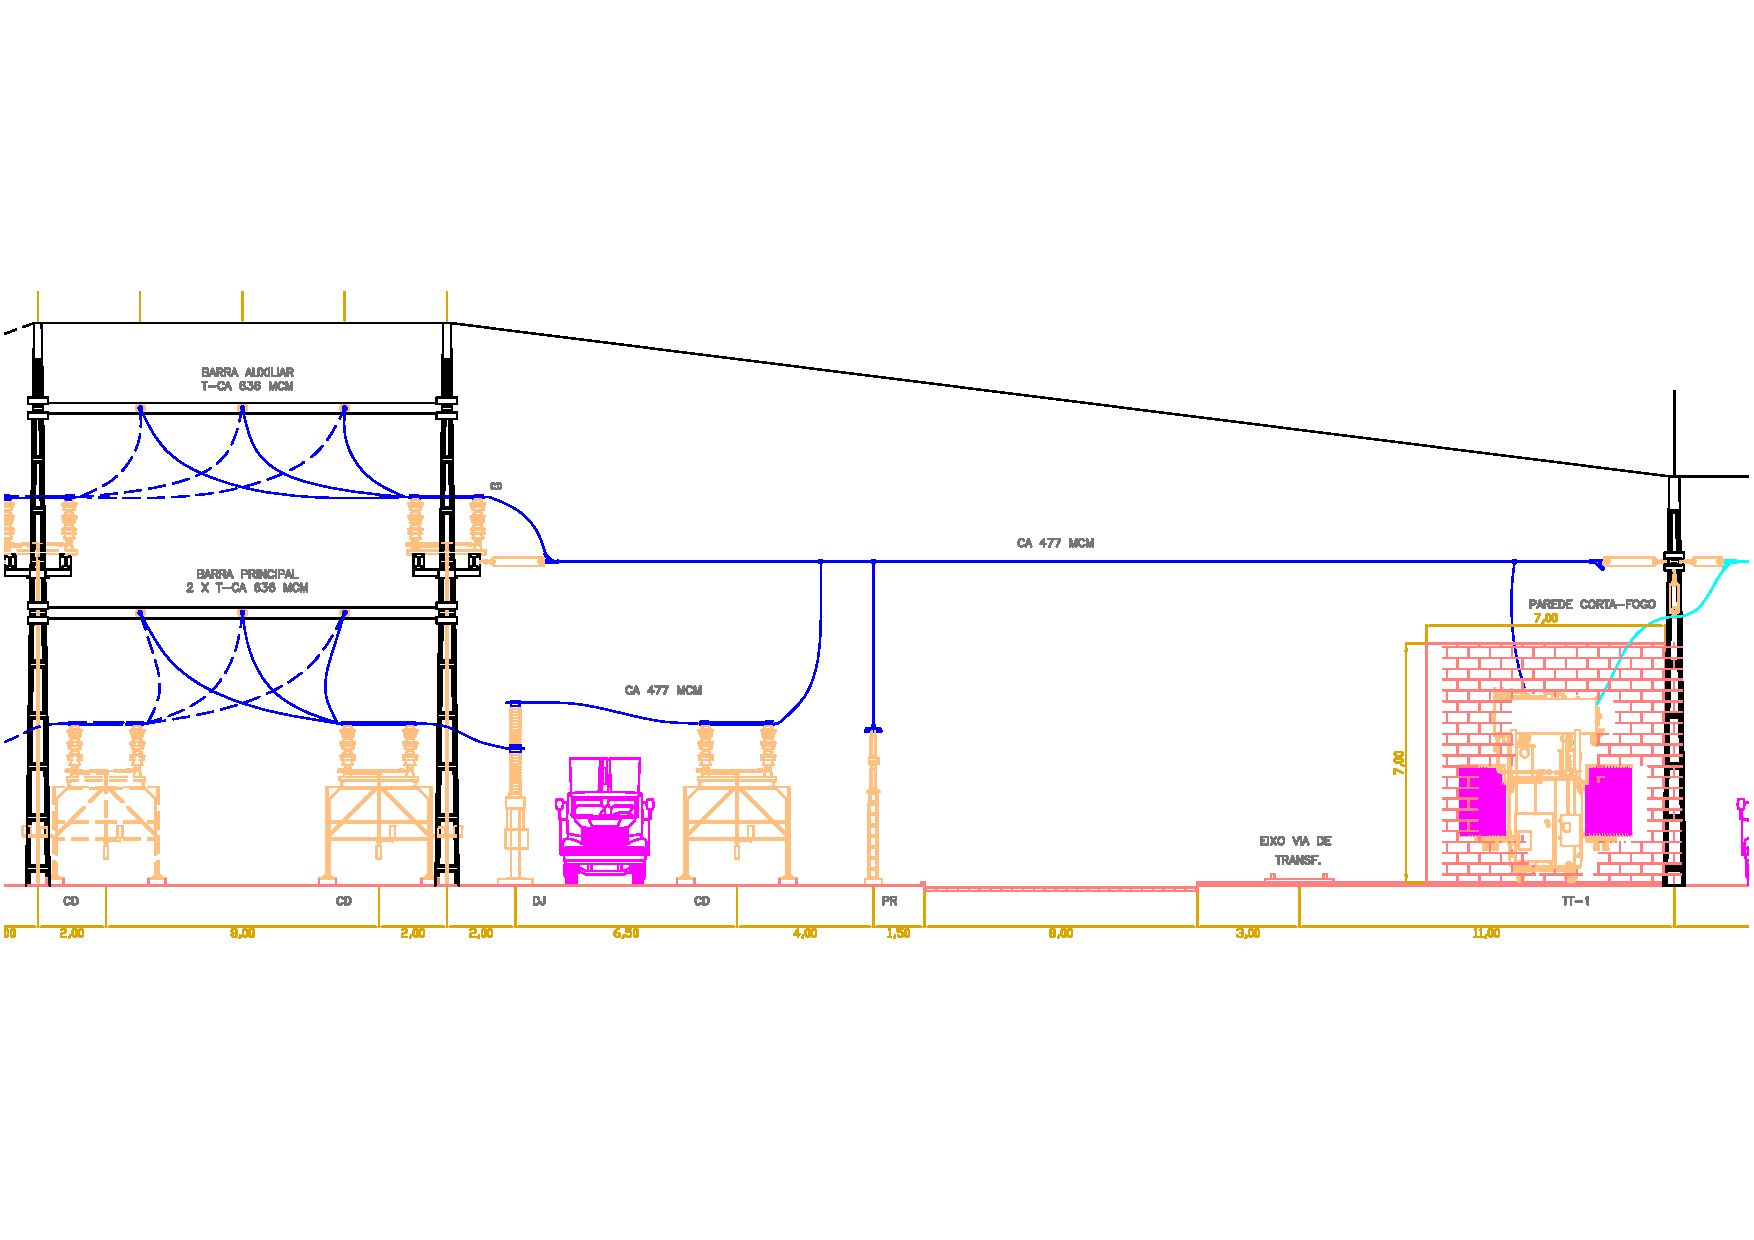
\includegraphics[width=108mm]{CTcorte.pdf}
				\legend{Fonte: Cedido por Celesc S.A. - Subestação Concórdia São Cristóvão - 138/34/13,8kV}
				\label{fig:CTcorte}
				\end{figure}
		\subsection{Alimentador (AL)}
			Os alimentadores são os vãos de ramificação geralmente de saída ligados no setor de baixa do qual a energia elétrica diverge para abastecimento de uma carga. Neste \textit{bays} é utilizado o religador (RL) como dispositivo de proteção como mostrado na \autoref{fig:UNAL}.\par
			\begin{figure}[!b]
				\caption{Diagrama unifilar de um alimentador}
				\centering
				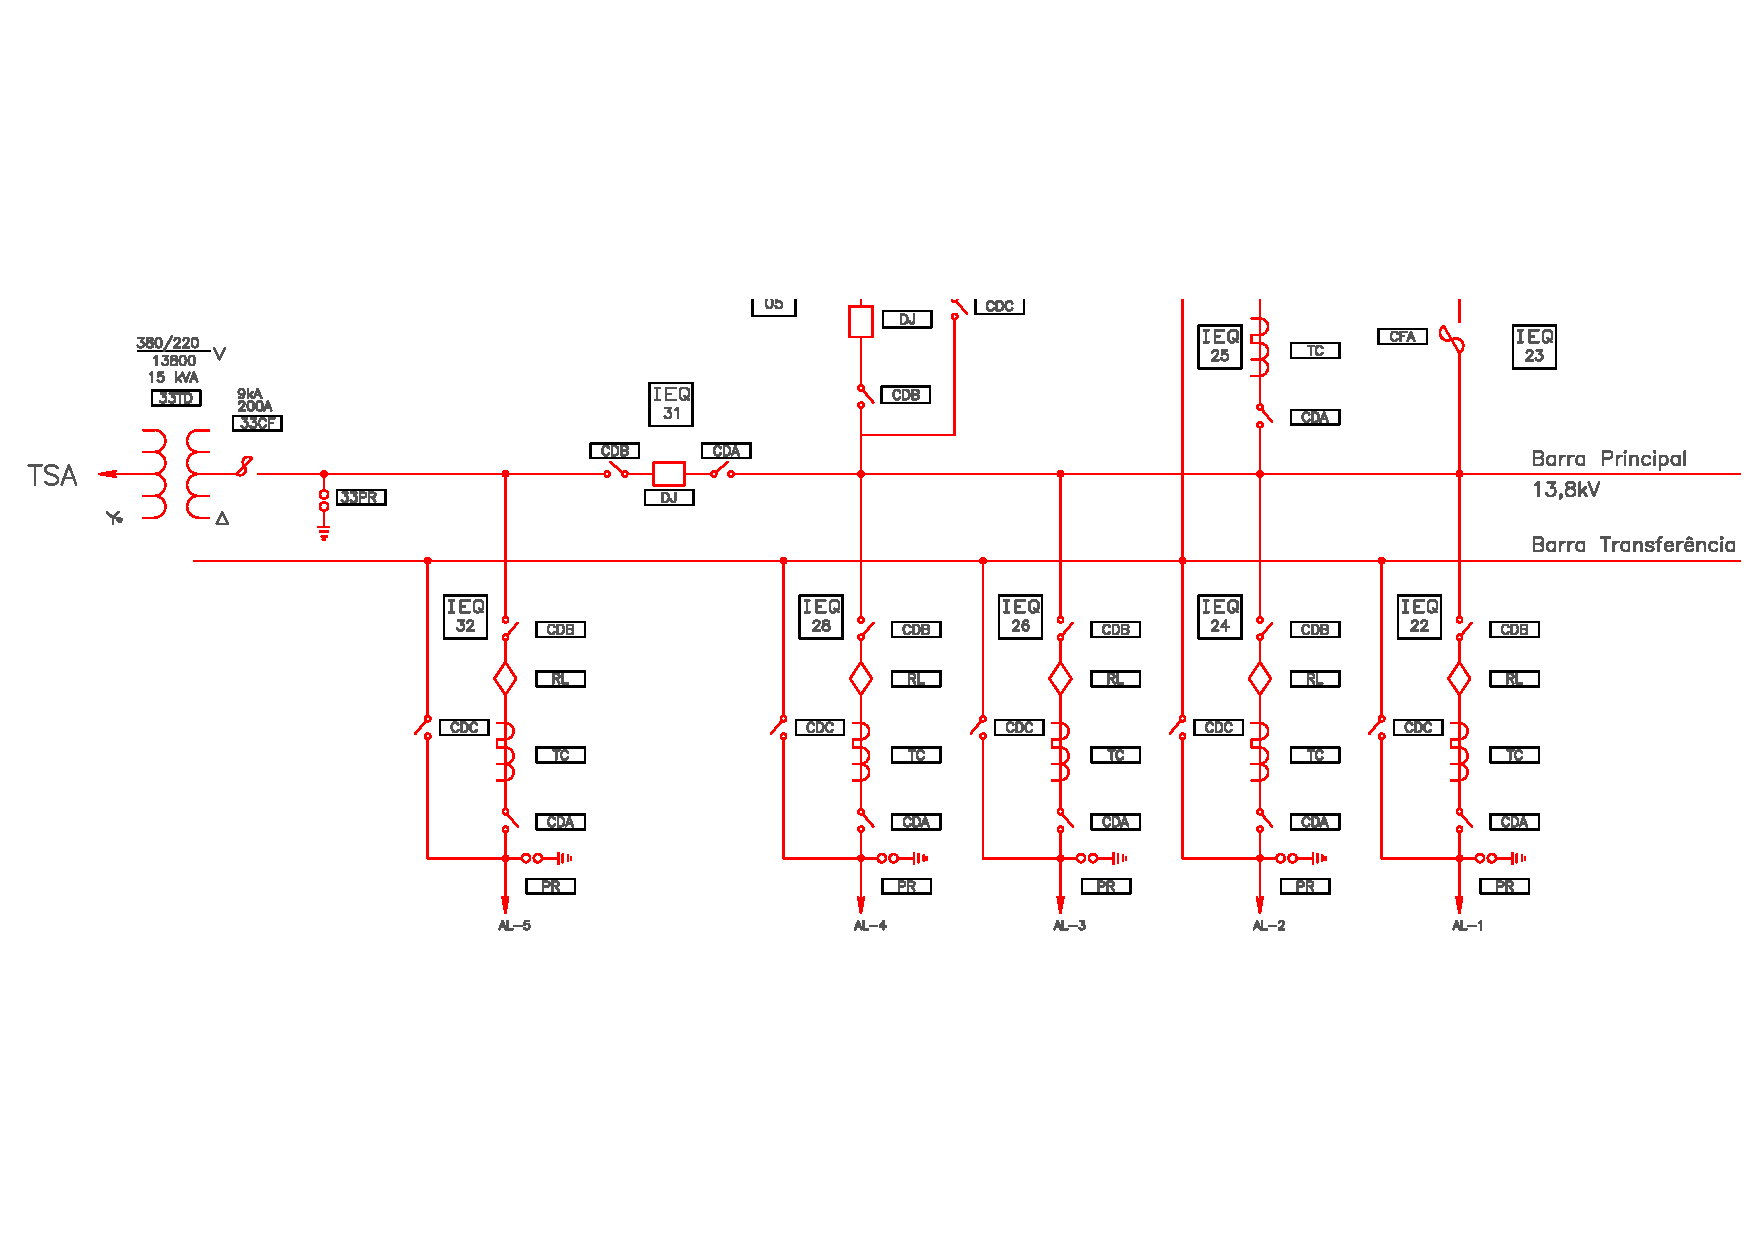
\includegraphics[width=108mm]{UNAL.pdf}
				\legend{Fonte: Do autor}
				\label{fig:UNAL}
				\end{figure}
		\subsection{Interligação de Barramentos (IB)}
			\label{sec:IB}
			Quando se faz necessário a substituição ou manutenção de um disjuntor de uma entrada de linha ou o religador de um alimentador, entra em ação como substituto o disjuntor ou religador de transferência comumente chamado de TIE que inglês tem o significado de "amarrar" ou "vincular" as duas barras para transferir a função de proteção ou controle.\par
			Outra função pode ser chamada de interligação de barramento quando se deseja seccionar uma barra (feita sempre no barramento principal), que pode ser tanto por uma seccionadora, ou quando se prioriza a confiabilidade, através de um disjuntor. Embora o seccionamento não elimine por completo o risco de perda total da subestação devido à ocorrência de falhas, a sua probabilidade é substancialmente reduzida, pois somente uma falha no disjuntor de seccionamento é que provocará este evento severo. A flexibilidade para a manutenção das secções de barras tem uma sensível melhora, mantendo-se a subestação parcialmente em operação.\par
			A \autoref{fig:UNIB} mostra um setor de baixa de uma subestação onde o barramento principal se encontra seccionado por um disjuntor, isto é feito nos casos onde o setor ultrapassa o número de quatro alimentadores, o vão com número IEQ 25 também mostra o TIE composto por um religador, quando necessário a manutenção ou substituição dos religadores do alimentador.\par
			\begin{figure}[!htb]
				\caption{Diagrama Unifilar de um setor de baixa tensão de uma subestação}
				\centering
				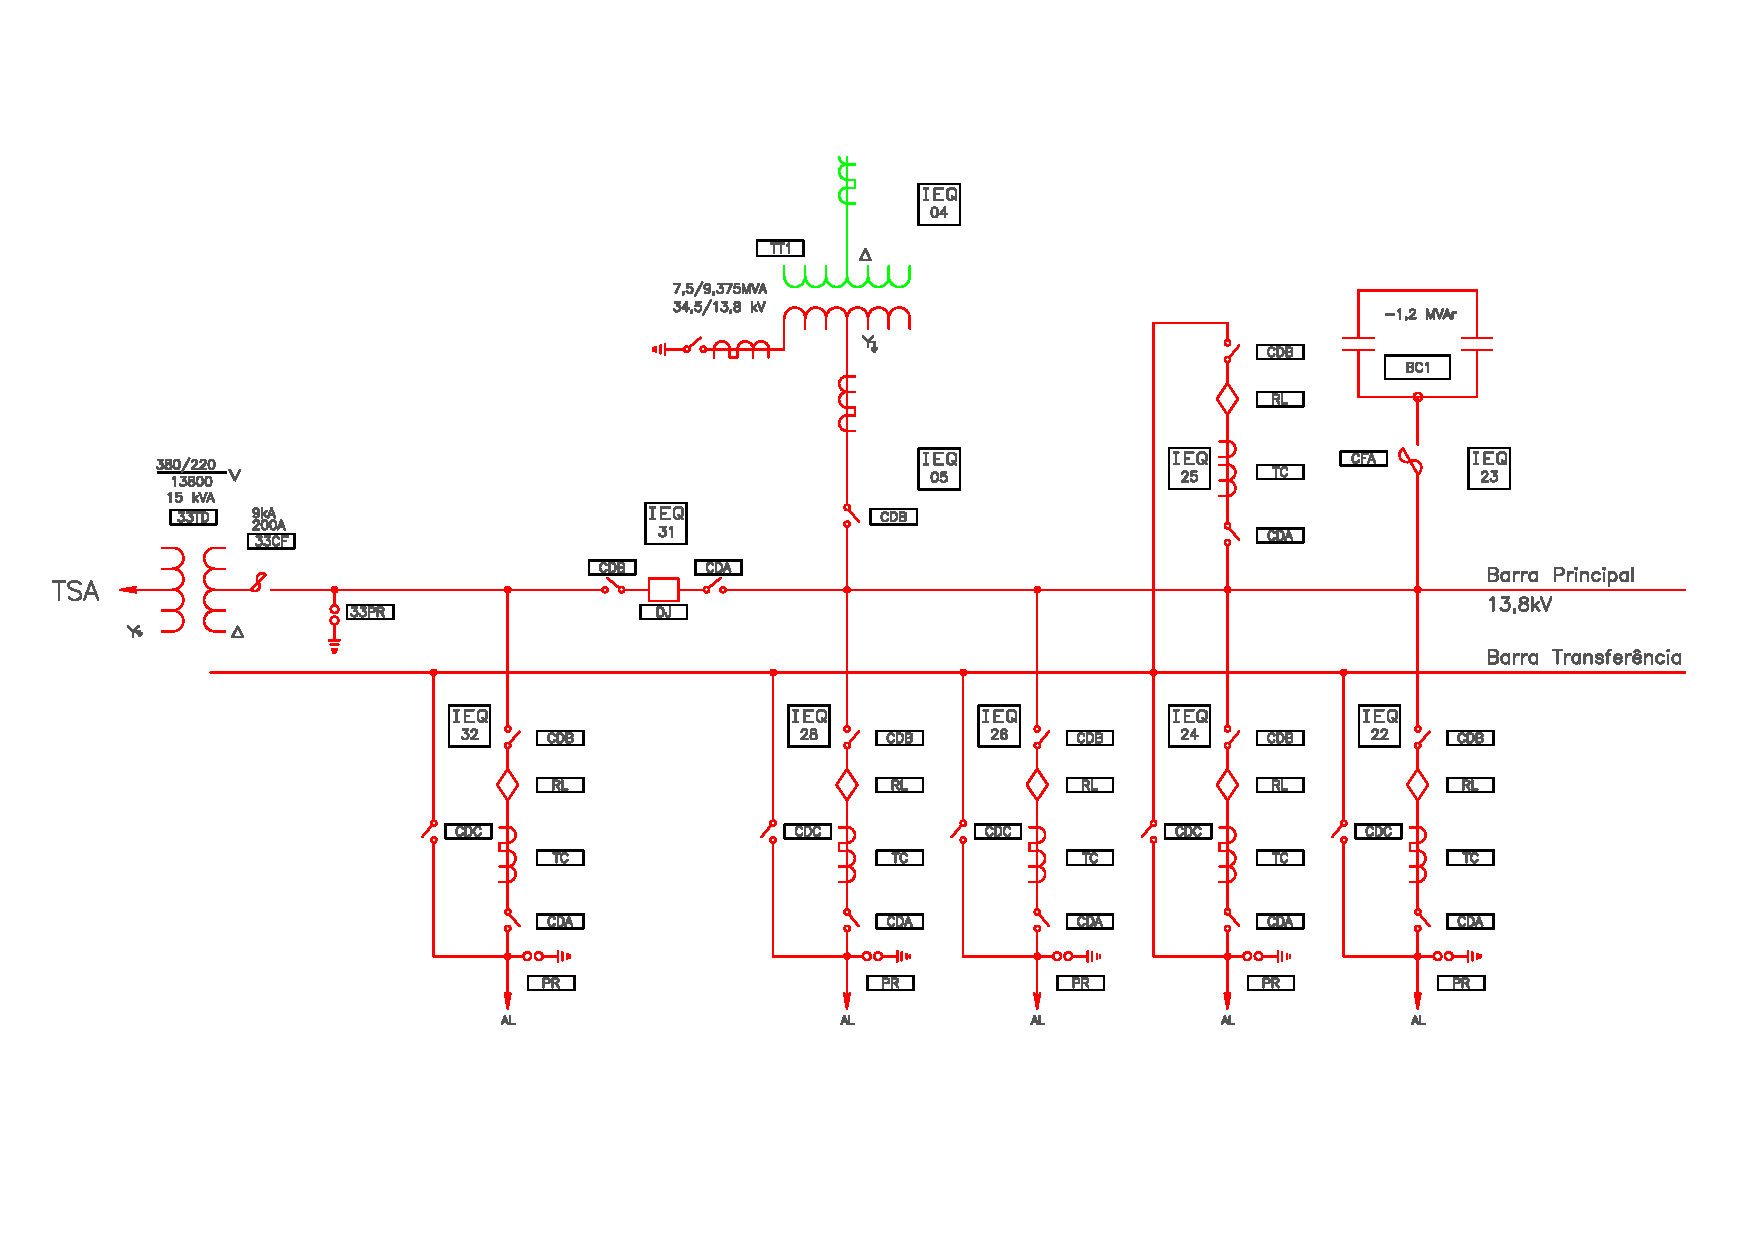
\includegraphics[width=10.8cm]{IB.pdf}
				\legend{Fonte: Do autor}
				\label{fig:UNIB}
				\end{figure}			
	\section{Configurações de barra}
		Segundo \citeonline{guiaprojetoSE} a configuração de barra utilizada deverá levar em consideração fatores de confiabilidade, custo simplicidade construtiva flexibilidade operativa facilidade de manutenção e facilidade de expansão. Já \citeonline{book:equipAT} considera que se a configuração de barra estiver abaixo das necessidades do sistema pode fragilizá-la, agora se estiver acima haverá investimentos ociosos. Contudo, a decisão se dará principalmente pela posição de dois principais equipamentos, o disjuntor representado como DJ, e as chaves seccionadoras CD mostradas nos esquemas a seguir.
		\subsection{Barra Simples (BS)}
			A \autoref{fig:BS} apresenta a configuração em barra simples, trata-se das mais básicas configurações de barra utilizada em subestações de pequeno porte em média e alta tensão, aplicadas em subestações de distribuição ou subestações industriais.\par
			Já para \citeonline{materialhaffner} são citadas os \textit{tradeoff} a seguir:\par
			As vantagens são de menor custo em uma menor área, instalação e manobras simples (ligar e desligar circuitos alimentadores e entradas de linha).\par
			As desvantagens são que podem ser usadas quando as cargas podem ser interrompidas e de as falha, ampliação, ou manutenção no barramento implica em desligamento da linha, e consequente sobrecarga da subestação, caso seja uma entrada de linha ou interrupção do fornecimento dos consumidores caso seja um alimentador.\par
			Como mostrado na entrada de linha 1 da \autoref{fig:BS}, pode-se adicionar uma chave seccionadora CDC para melhoria do arranjo com função de \textit{bypass}, ou seja, passagem direta da energia, entretanto corre risco de caso esta chave CDC estar acionada expor a subestação a falhas.\par 
			\begin{figure}[!htb]
				\caption{Configuração Barra Simples}
				\centering
				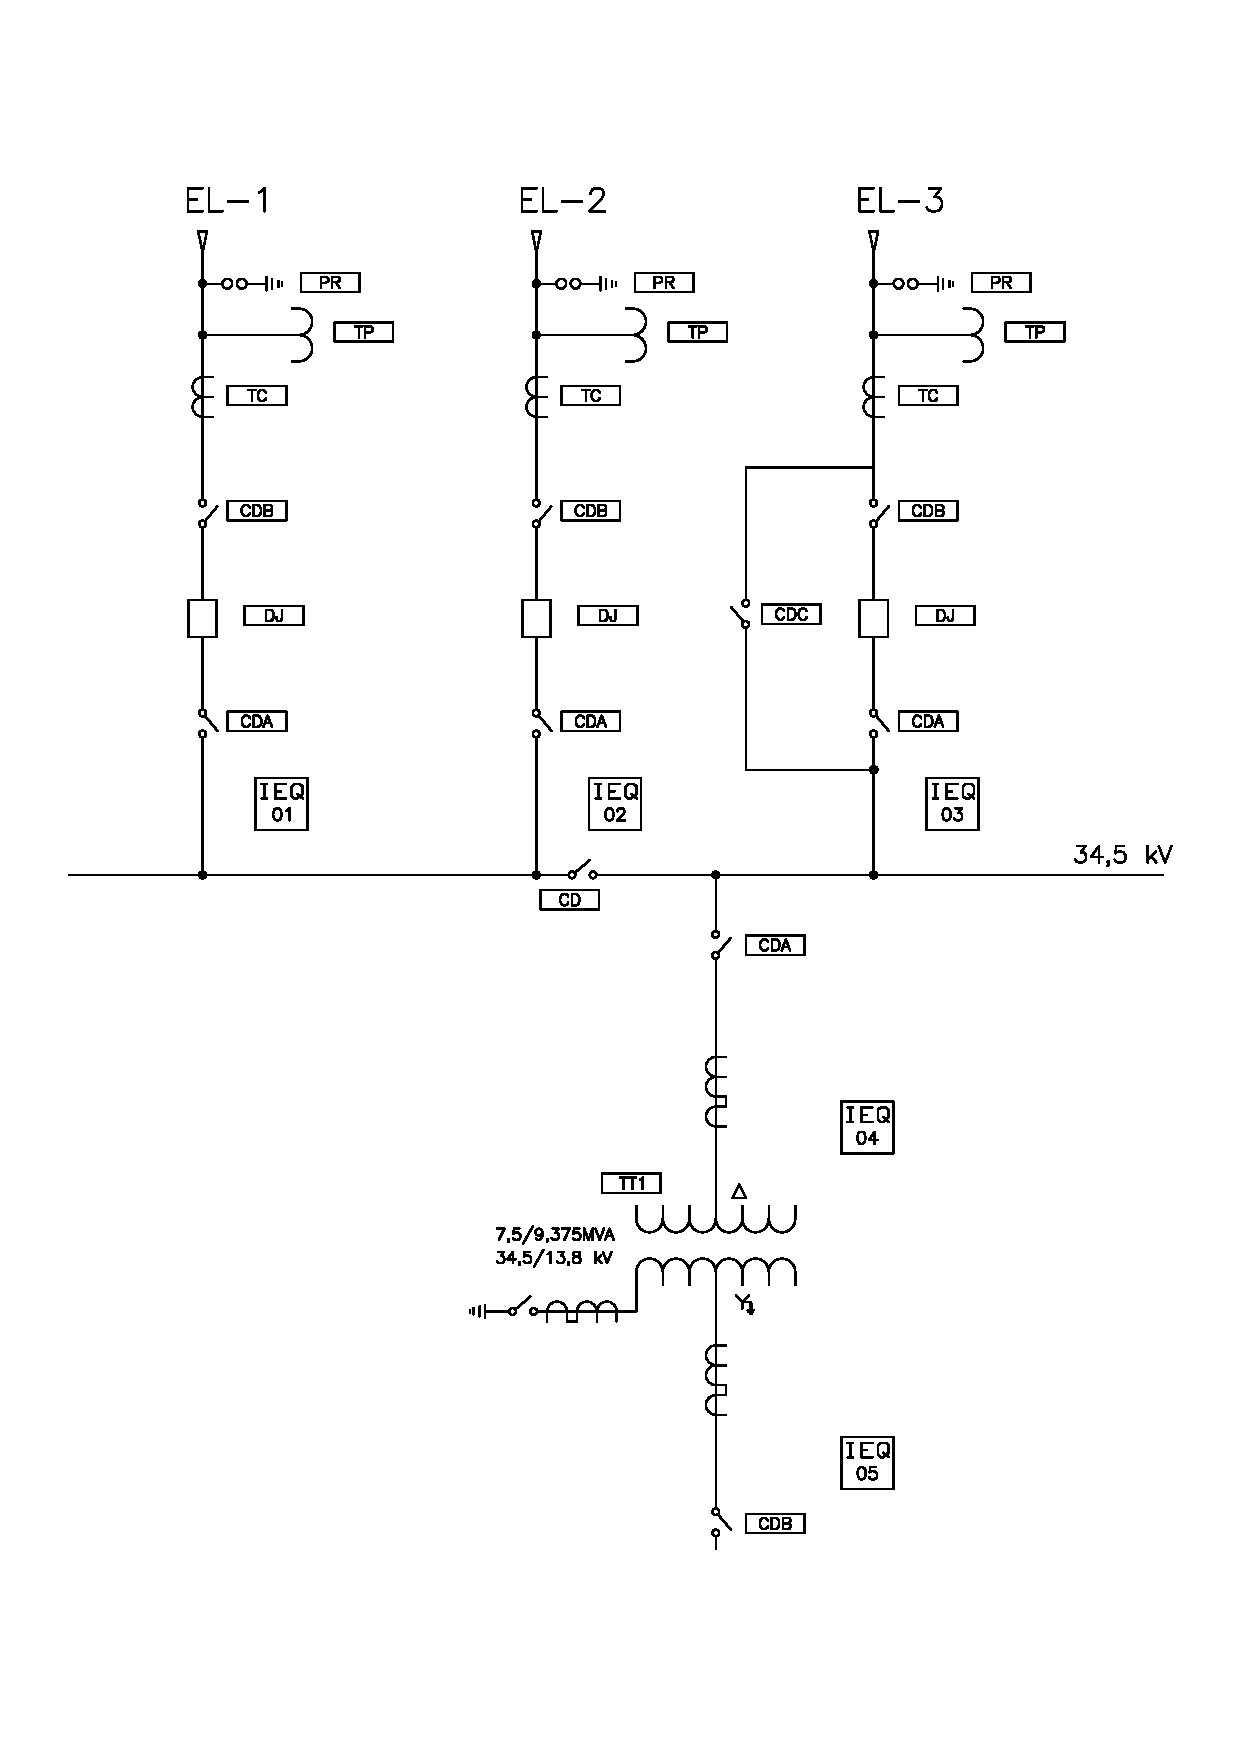
\includegraphics[width=10.8cm]{01BS.pdf}
				\legend{Fonte: Do autor}
				\label{fig:BS}
				\end{figure}
		\subsection{Barra Principal e Transferência (BP+T)} \label{sec:BPT}
			A \autoref{fig:BPT} apresenta a adição de uma barra de transferência ou também chamada de barra auxiliar, que permite a substituição ou manutenção de qualquer disjuntor sem o desligamento de qualquer linha. Nesta configuração é necessário todavia a adição do TIE, com função de interligação das barras e substituição da proteção para a linha em manutenção como citado na \autoref{sec:IB}.\par
			As vantagens são de baixo custo, qualquer disjuntor pode ser retirado de serviço para manutenção e os equipamentos podem ser conectados e desconectados à barra principal sem muitas dificuldades.\par
			As desvantagens são o custo de um disjuntor extra para conexão com outra barra, manobras relativamente complicadas para colocar um disjuntor em manutenção, falhas num barramento ou num disjuntor resulta no desligamento da subestação e a barra de transferência opera cerca de toda sua vida útil desenergizada.\par
			\begin{figure}[!htb]
				\caption{Configuração Barra Principal e Transferência}
				\centering
				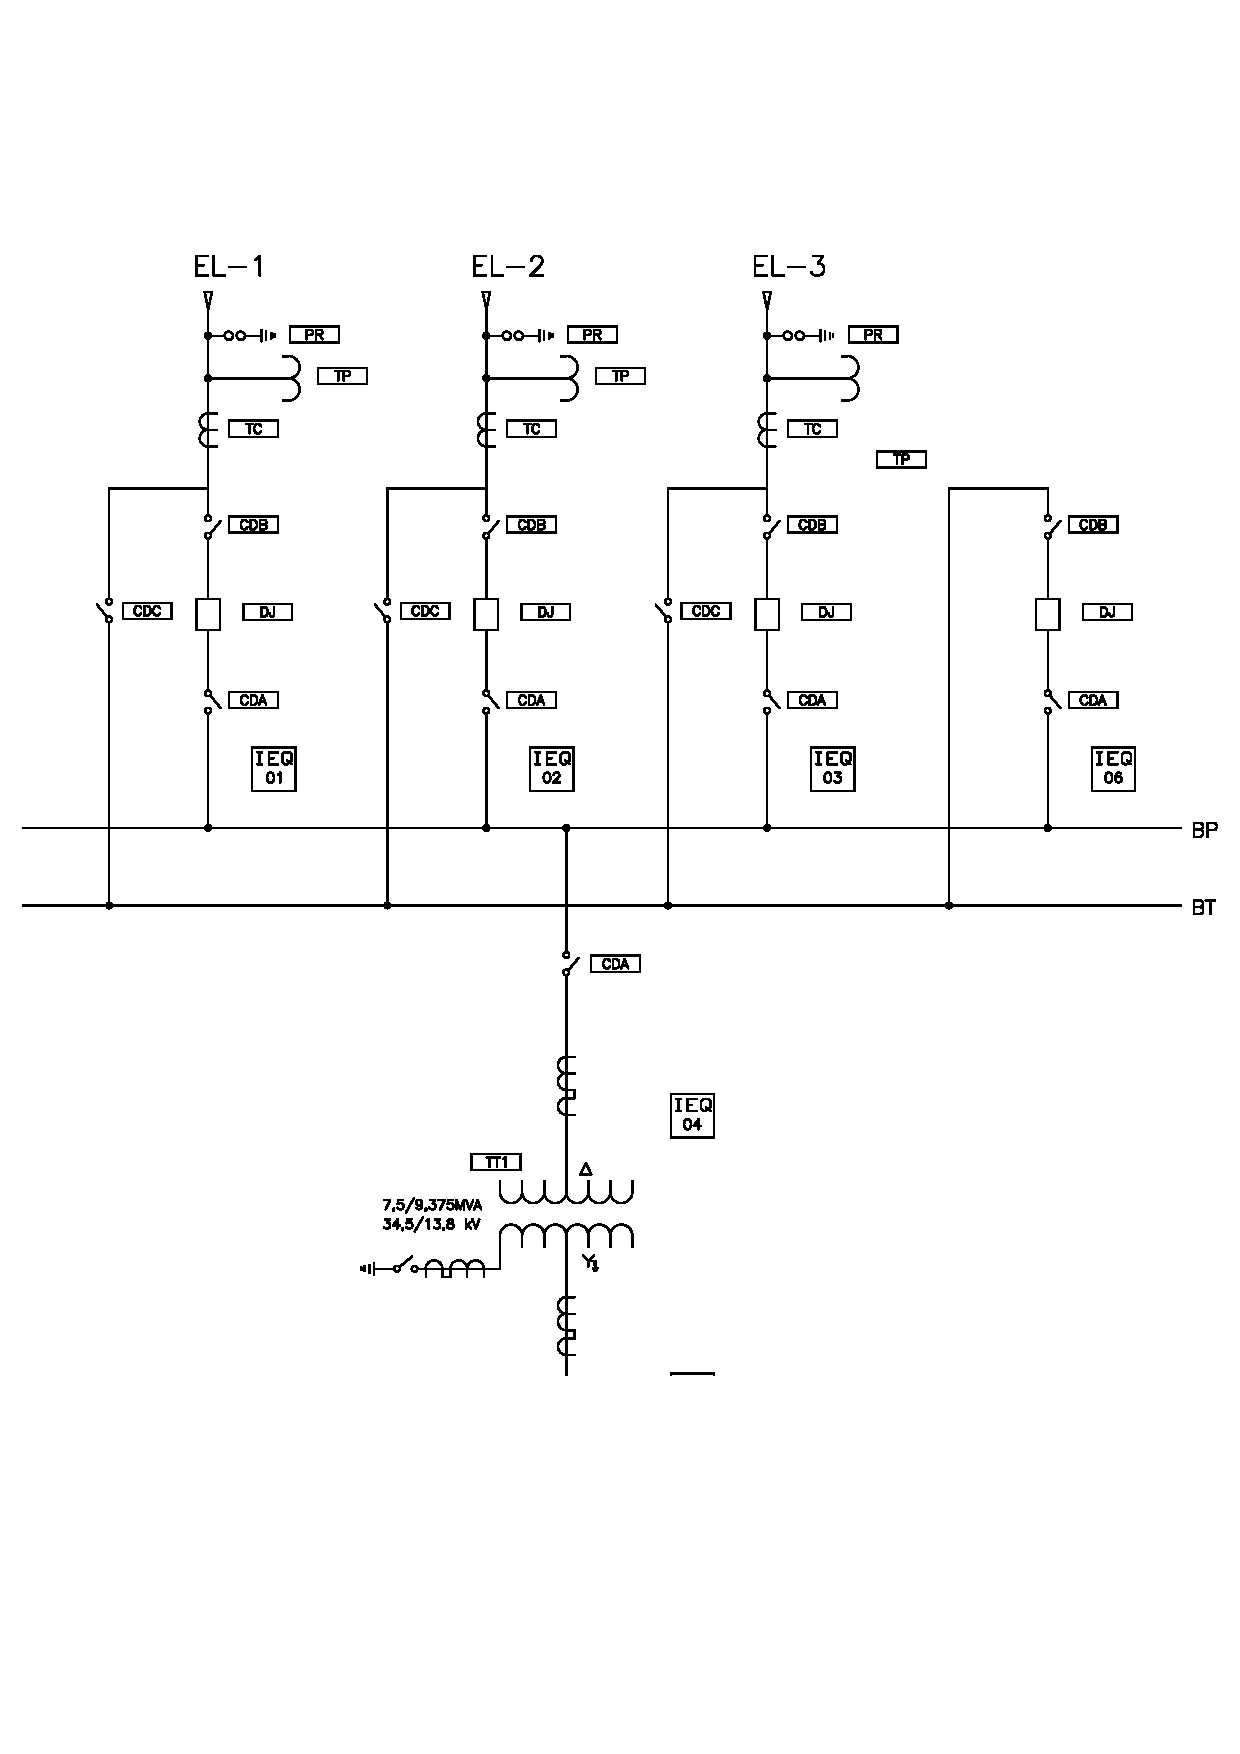
\includegraphics[width=10.8cm]{02BPT.pdf}
				\legend{Fonte: Do autor}
				\label{fig:BPT}
				\end{figure}
%		\subsection{Barra Principal Seccionada e Transferência (BPS+T)}
		\subsection{Barra Dupla com Disjuntor Simples a Três, Quatro e Cinco Chaves (BD-Ds-3 ch)}
			A \autoref{fig:BDs} apresenta três tipos de entrada de linha, a três, quatro e cinco chaves conectados a duas barras que ao contrário da \autoref{sec:BPT}, apresenta estas duas barras energizadas. O direcionamento é feito por meio das chaves seccionadoras das entradas de linha para separação de zona de proteção.\par
			Na entrada de linha (EL-1) com três chaves a inexistência de chaves de \textit{bypass}, a manutenção ou reparos em disjuntores retira de operação o circuito do sistema. Em sistemas em malha (malhado) ou redundantes, este fato torna-se irrelevante. Ainda, não ocorre a perda de configuração normal, minimizando os riscos do sistema. Na maior parte dos casos que se utiliza o \textit{bypass}, a configuração perdida e o sistema fragilizado.\par
			Na entrada de linha (EL-2) com quatro chaves é adicionado uma chave \textit{bypass} de forma que o disjuntor da entrada de linha possa ser liberado para manutenção e reparos sem que seja necessário desligar o circuito da linha. Neste caso se aproveita a operação da barra dupla e uma das barras, escolhida previamente, utiliza-se como barra de transferência, e dedicada a um \textit{bay}. Neste caso é possível liberar apenas um disjuntor de cada vez, ou seja, a proteção é para apenas uma linha.\par
			Segundo \citeonline{book:equipAT} a sequência de manobras para quatro chaves é: remanejar os circuitos para a barra exclusiva de operação (B1), exceto o do \textit{bay} a ser transferido que deve ser conectado à barra B2; fechar a chave de \textit{bypass} do referido \textit{bay}, abrir o disjuntor a ser liberado e abrir as suas chaves de isolamento.\par
			Ainda sobre a configuração a quatro chaves, esta sendo a mais utilizada no brasil para rede básica, otimiza os investimentos, pois apenas duas chaves operam normalmente abertas.\par
			Na entrada de linha (EL-3) com cinco chaves, segundo \cite{book:equipAT} é utilizado em subestações de $138kV$ e $230kV$. Apesar de possuir um grau de flexibilidade com aumento de uma chave com relação à configuração anterior, adicionar uma chave significa aumentar o número de intertravamentos e possibilidade de falhas, já que não há como definir a barra de transferência previamente e por apresentar maior de equipamentos e área energizados.\par
			Geralmente é utilizado apenas um tipo de configuração das três apresentadas a seguir, porém há casos específicos onde podem ser utilizados soluções mistas quando trata-se de subestações envolvendo geradores que passam desligados parte do tempo que reduzem a necessidade de chaves \textit{bypass}, neste caso utiliza-se a configuração a três chaves e os alimentadores a quatro chaves.\par
			\begin{figure}[!htb]
				\caption{Configuração Barra Dupla com Disjuntor Simples a Três, Quatro e Cinco Chaves}
				\centering
				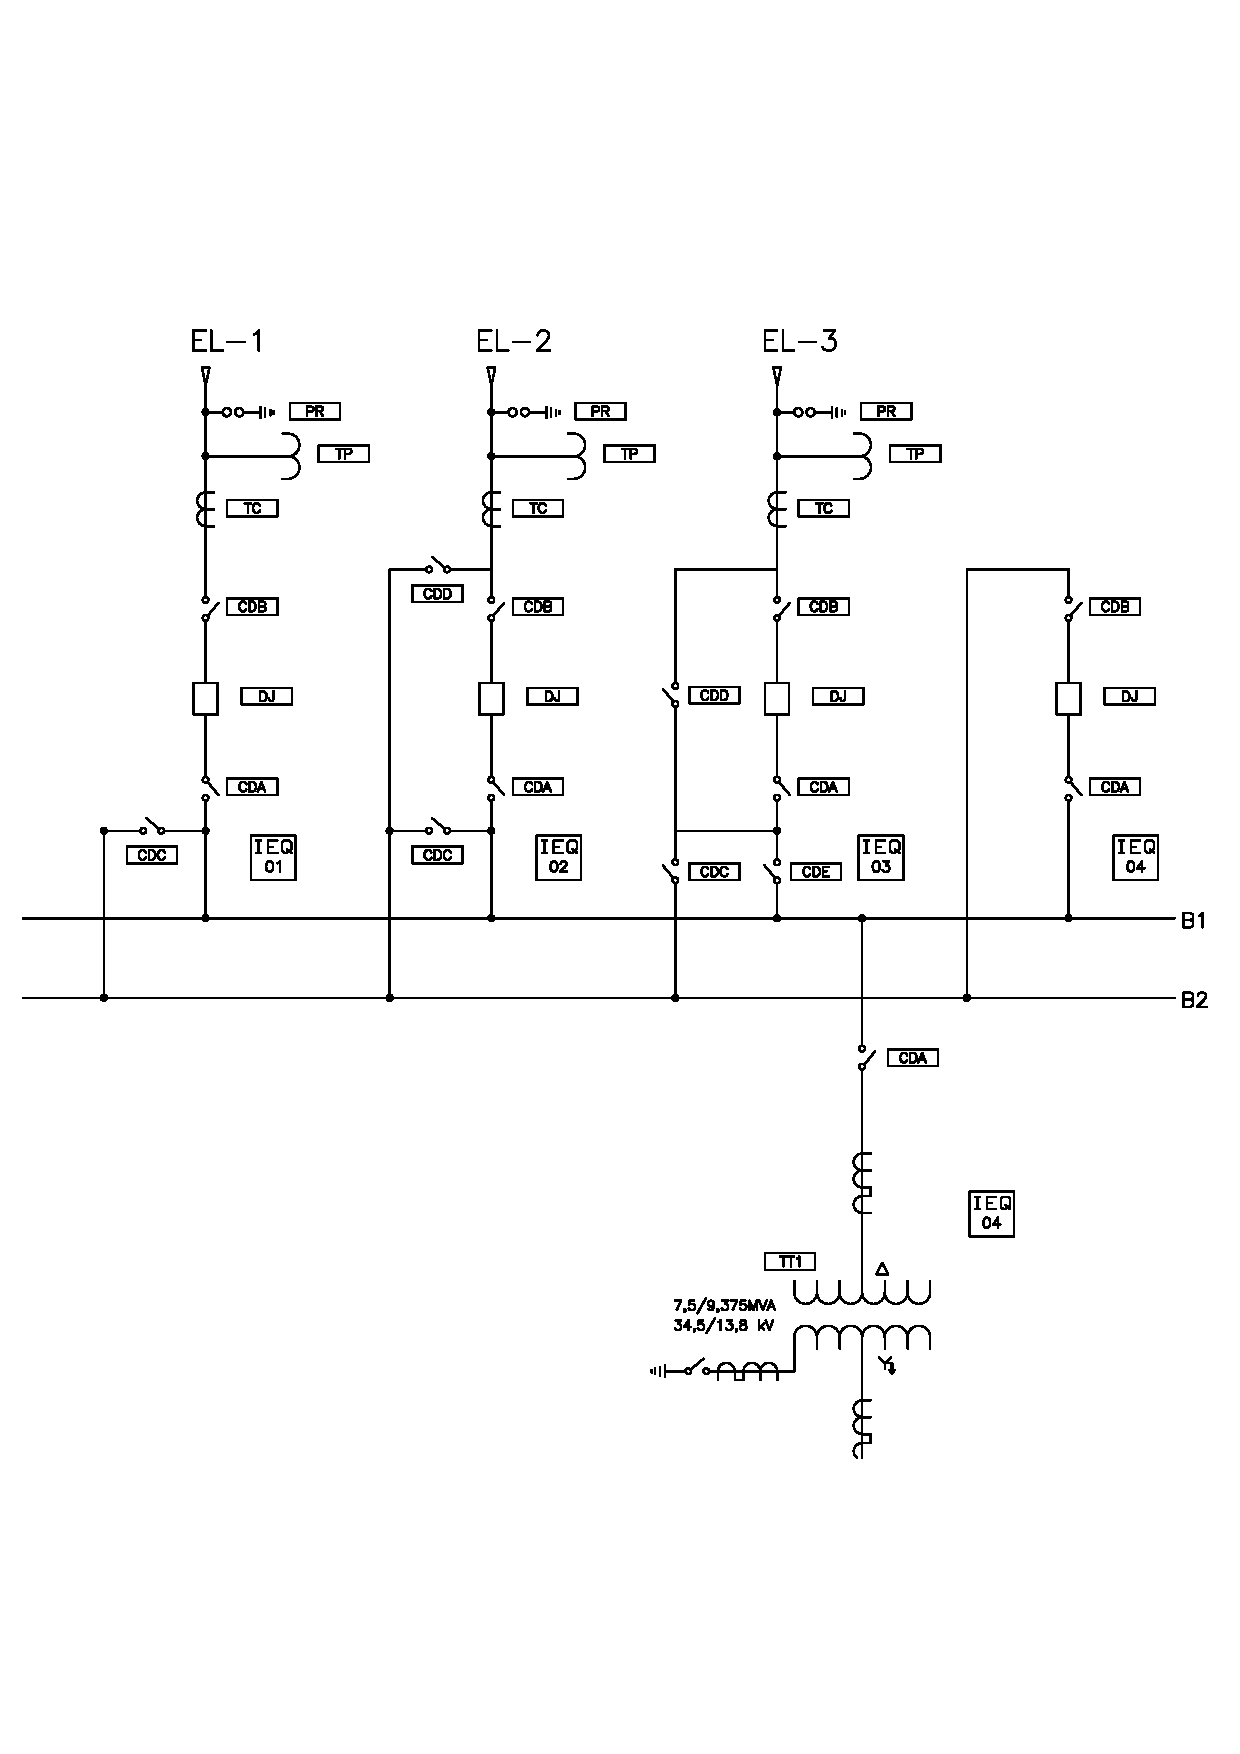
\includegraphics[width=10.8cm]{03BDs.pdf}
				\legend{Fonte: Do autor}
				\label{fig:BDs}
				\end{figure}
%		\subsection{Barra Dupla com Disjuntor Simples a Quatro Chaves (BD-Ds-4 ch)}
%		\subsection{Barra Dupla com Disjuntor Simples a Cinco Chaves (BD-Ds-5 ch)}
%		\subsection{Barra Dupla com Disjuntor Simples a Três e Quatro (Chaves BD-Ds-3 e 4 ch)}
%		\subsection{Barra Dupla e Transferência com Disjuntor Simples a Três e Quatro Chaves (BD+T)}
%		\subsection{Barra Dupla Seccionadas com Disjuntor Simples a Quatro Chaves (BDS-Ds-4 ch)}
		\subsection{Anel Simples (AN)}
			A \autoref{fig:AN} apresenta a configuração em anel simples, onde observa-se a conexão de quatro ramos por meio de um laço elétrico formado por disjuntores, esta configuração permite saída de operação de um disjuntor sem interromper o fornecimento de energia dos outros ramos. Possui a vantagem de ser econômica e simples, porém, expõe a sistema a ocorrências externas.\par
			Segundo \citeonline{guiaprojetoSE} a configuração possui a desvantagem de os disjuntores serem dimensionados para o dobro da corrente de curto-circuito dos circuitos de alimentação.\par
			\begin{figure}[!htb]
				\caption{Configuração Anel Simples}
				\centering
				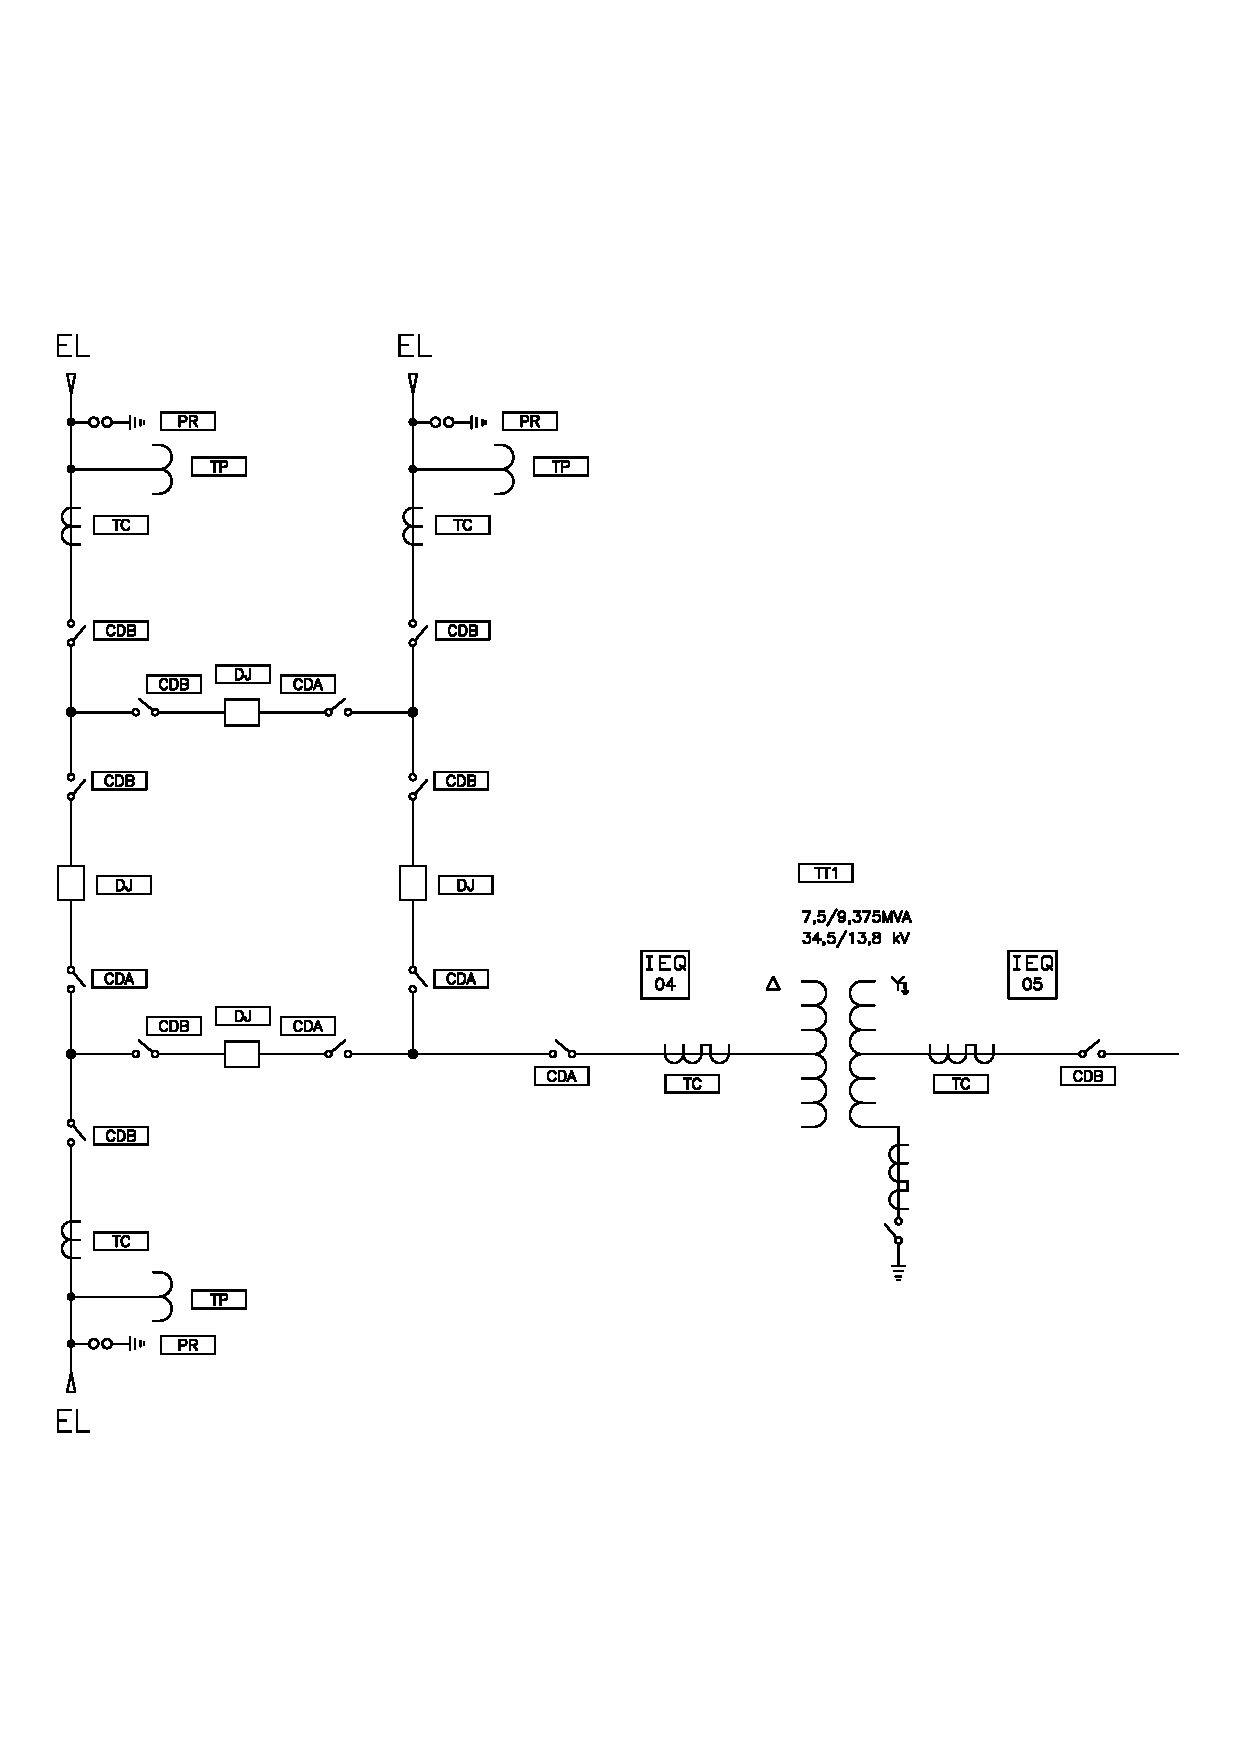
\includegraphics[width=10.8cm]{08AN.pdf}
				\legend{Fonte: Do autor}
				\label{fig:AN}
				\end{figure}
		\subsection{Anel Múltiplo (ANM)}
			A \autoref{fig:ANM} apresenta a configuração em anel múltiplo para subestações onde é necessário maior segurança e disponibilidade, presentes em subestações de 230kV, 345kV e 500kV.\par
			Ela possui a vantagem de ser mais econômica por apresentar oito conexões com apenas nove disjuntores, o laço elétrico adicionado conduz à estabilidade que minimiza a perda de configuração de configuração da subestação.\par
			As desvantagens está em dificuldade de projetos de sua expansão, possibilidade de ser necessário o cruzamento de circuitos que atrapalham na visualização de equipamentos durante ações de manutenções no pátio.\par
			Outro fato está da configuração não ser simétrica, pois há dois nós que são protegidos por três disjuntores enquanto que os demais por dois disjuntores. Segundo \citeonline{book:equipAT} neste caso não é recomendável conectar linhas de transmissão, geradores ou equipamentos de compensação de reativos que requeiram manobras frequentes, pois em uma ocorrência haverá separação dos circuitos e formação de ilhas elétricas com consequências severas para o sistema elétrico.\par
			\begin{figure}[!htb]
				\caption{Configuração Anel Múltiplo}
				\centering
				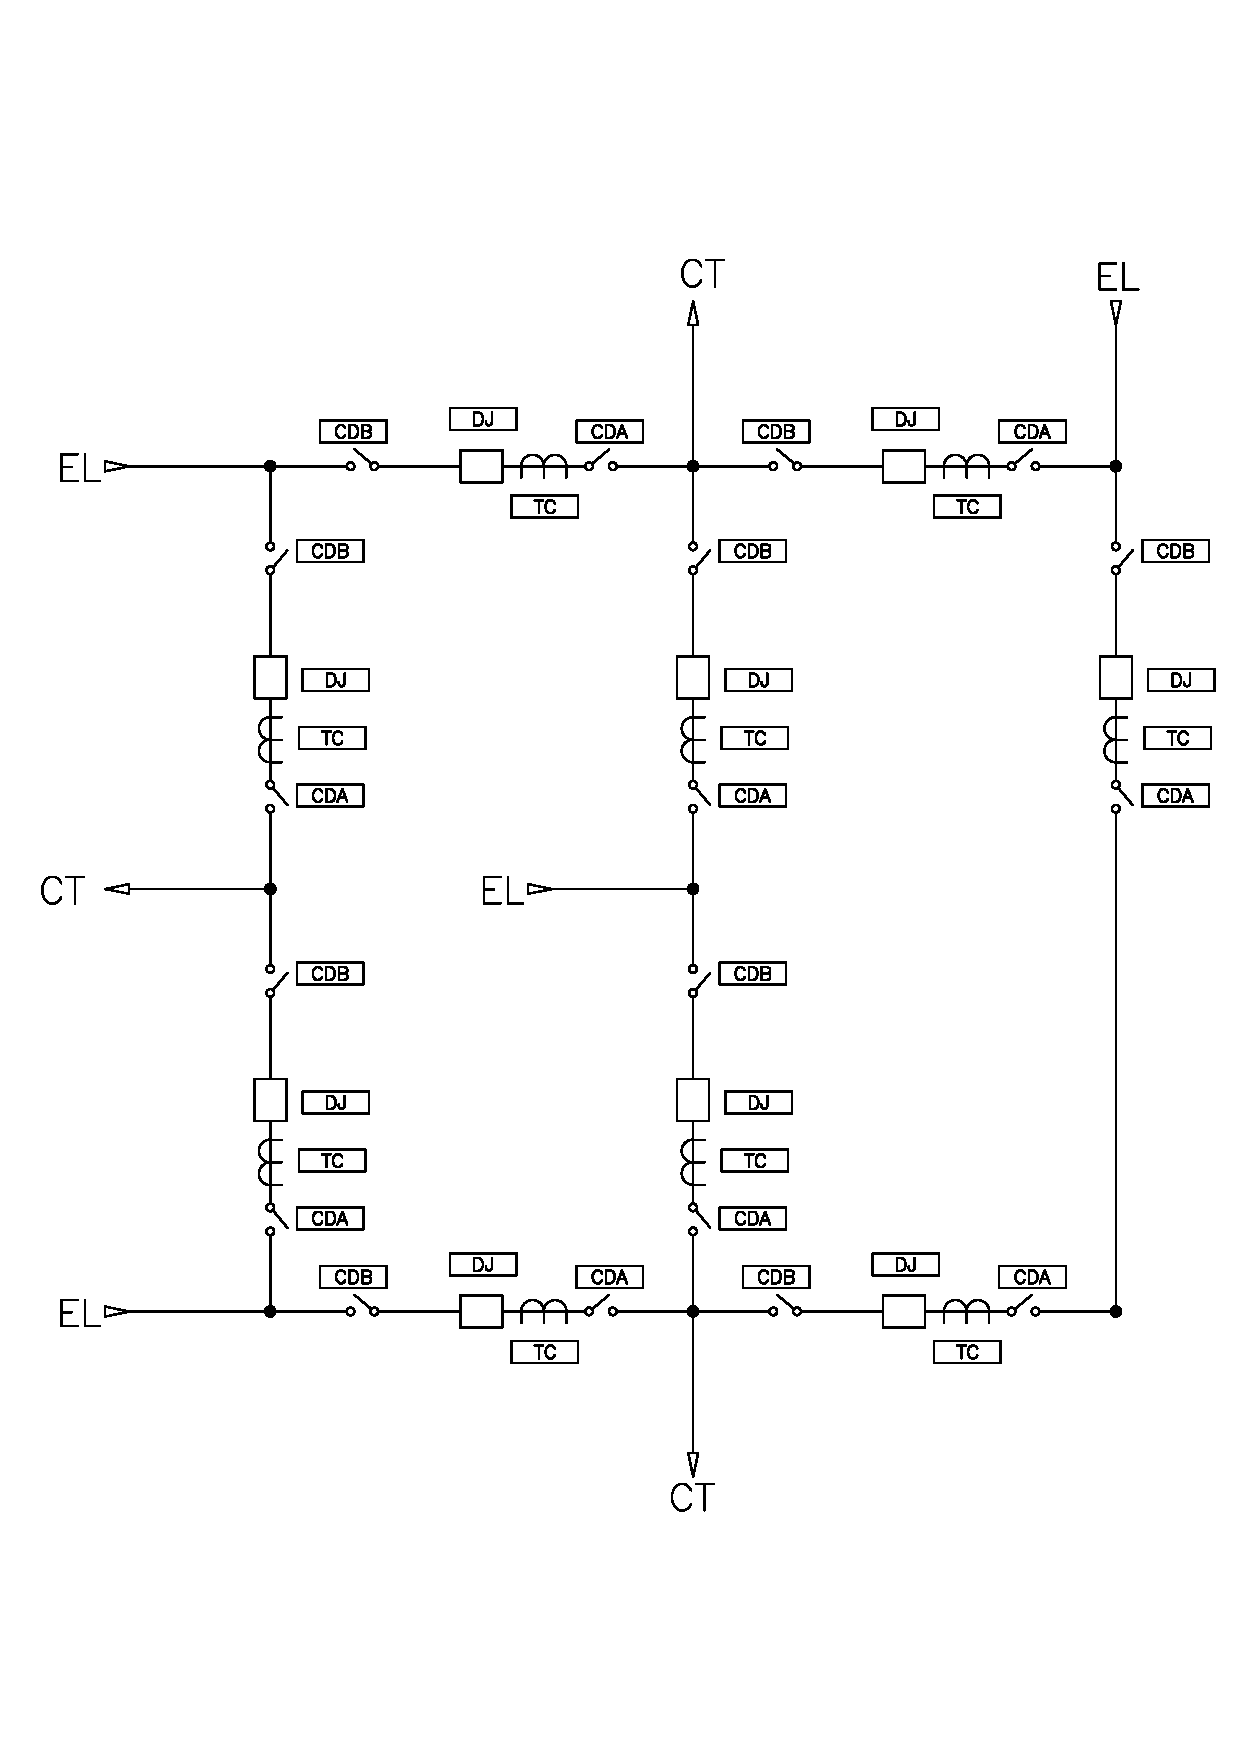
\includegraphics[width=10.8cm]{09ANM.pdf}
				\legend{Fonte: Do autor}
				\label{fig:ANM}
				\end{figure}
		\subsection{Barra Dupla com Disjuntor e Meio (BD-D1/2)}
			A \autoref{fig:BD-D1/2} mostra a configuração com disjuntor e meio que utiliza três disjuntores para conectar dois terminais, cada terminal é protegido por um disjuntor exclusivo mais um compartilhado entre os dois, deste modo, vem o nome de um disjuntor e meio. É utilizado quando a segurança é um fator essencial.\par
			Esta configuração se torna estável pois há menores perdas de configuração devido às ocorrências de falhas com a existência do segundo laço elétrico.\par
			Segundo \citeonline{book:equipAT} esta configuração, usual nas subestações acima de 345 kV do sistema elétrico brasileiro, possui boa flexibilidade operativa, facilidades para a sua expansão e fácil visualização dos equipamentos no pátio de manobras devido ao arranjo físico adotado: equipamentos instalados entre as barras. No entanto, comparativamente com outras configurações de barra, esta configuração é de custo relativamente elevado. Para a conexão de seis circuitos, são necessários nove disjuntores (um e meio por \textit{bay}), nove conjuntos de TC’s e 24 chaves seccionadoras. Portanto, é necessário realizar um balanço entre a real necessidade para o sistema elétrico e os investimentos para a sua implantação e evolução.\par
			\begin{figure}[!htb]
				\caption{Configuração Barra Dupla com Disjuntor e Meio}
				\centering
				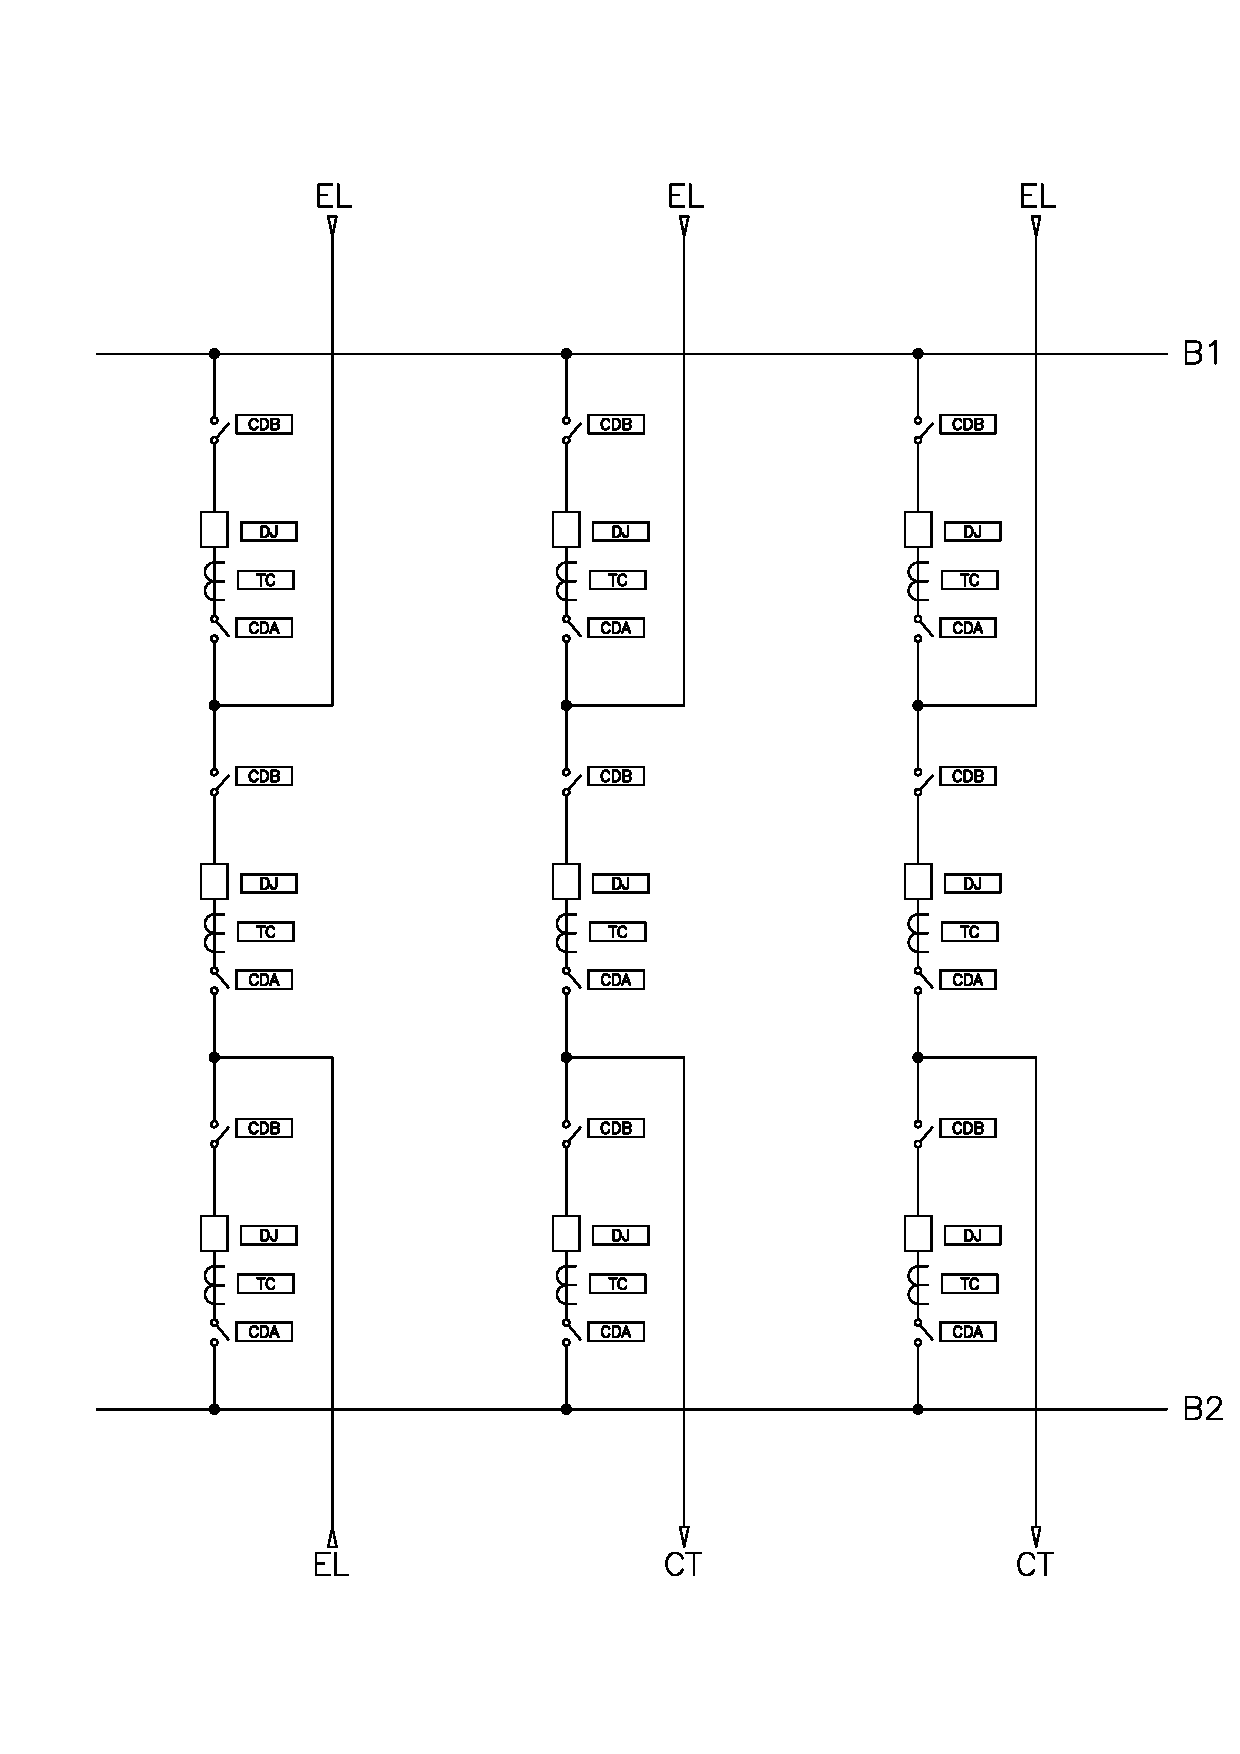
\includegraphics[width=10.8cm]{10BD-D1e2.pdf}
				\legend{Fonte: Do autor}
				\label{fig:BD-D1/2}
				\end{figure}
		\subsection{Barra Dupla com Disjuntor e Meio Modificado (BD-D1/2-M)}
			Com intuito de reduzir custos e resguardar uma ampliação que aumente a segurança no futuro neste exemplo é apresentado a mesma configuração de disjuntor e meio, mas com terminais conectados nas barras, com isso a configuração passa a ser um anel simples com seis terminais apresentado na \autoref{fig:BD-D1/2M}.\par
			Segundo \citeonline{book:equipAT} devem ser tomados dois cuidados: (i) o sistema de proteção deve permitir a rápida identificação da falha, separando falha na barra de falha nos autotransformadores conectados diretamente às barras, (ii) não devem ser conectados diretamente às barras linhas de transmissão elementos de compensação de reativos (bancos de capacitores ou de reatores), ou unidades geradoras.\par
			\begin{figure}[!htb]
				\caption{Configuração Barra Dupla com Disjuntor e Meio Modificado}
				\centering
				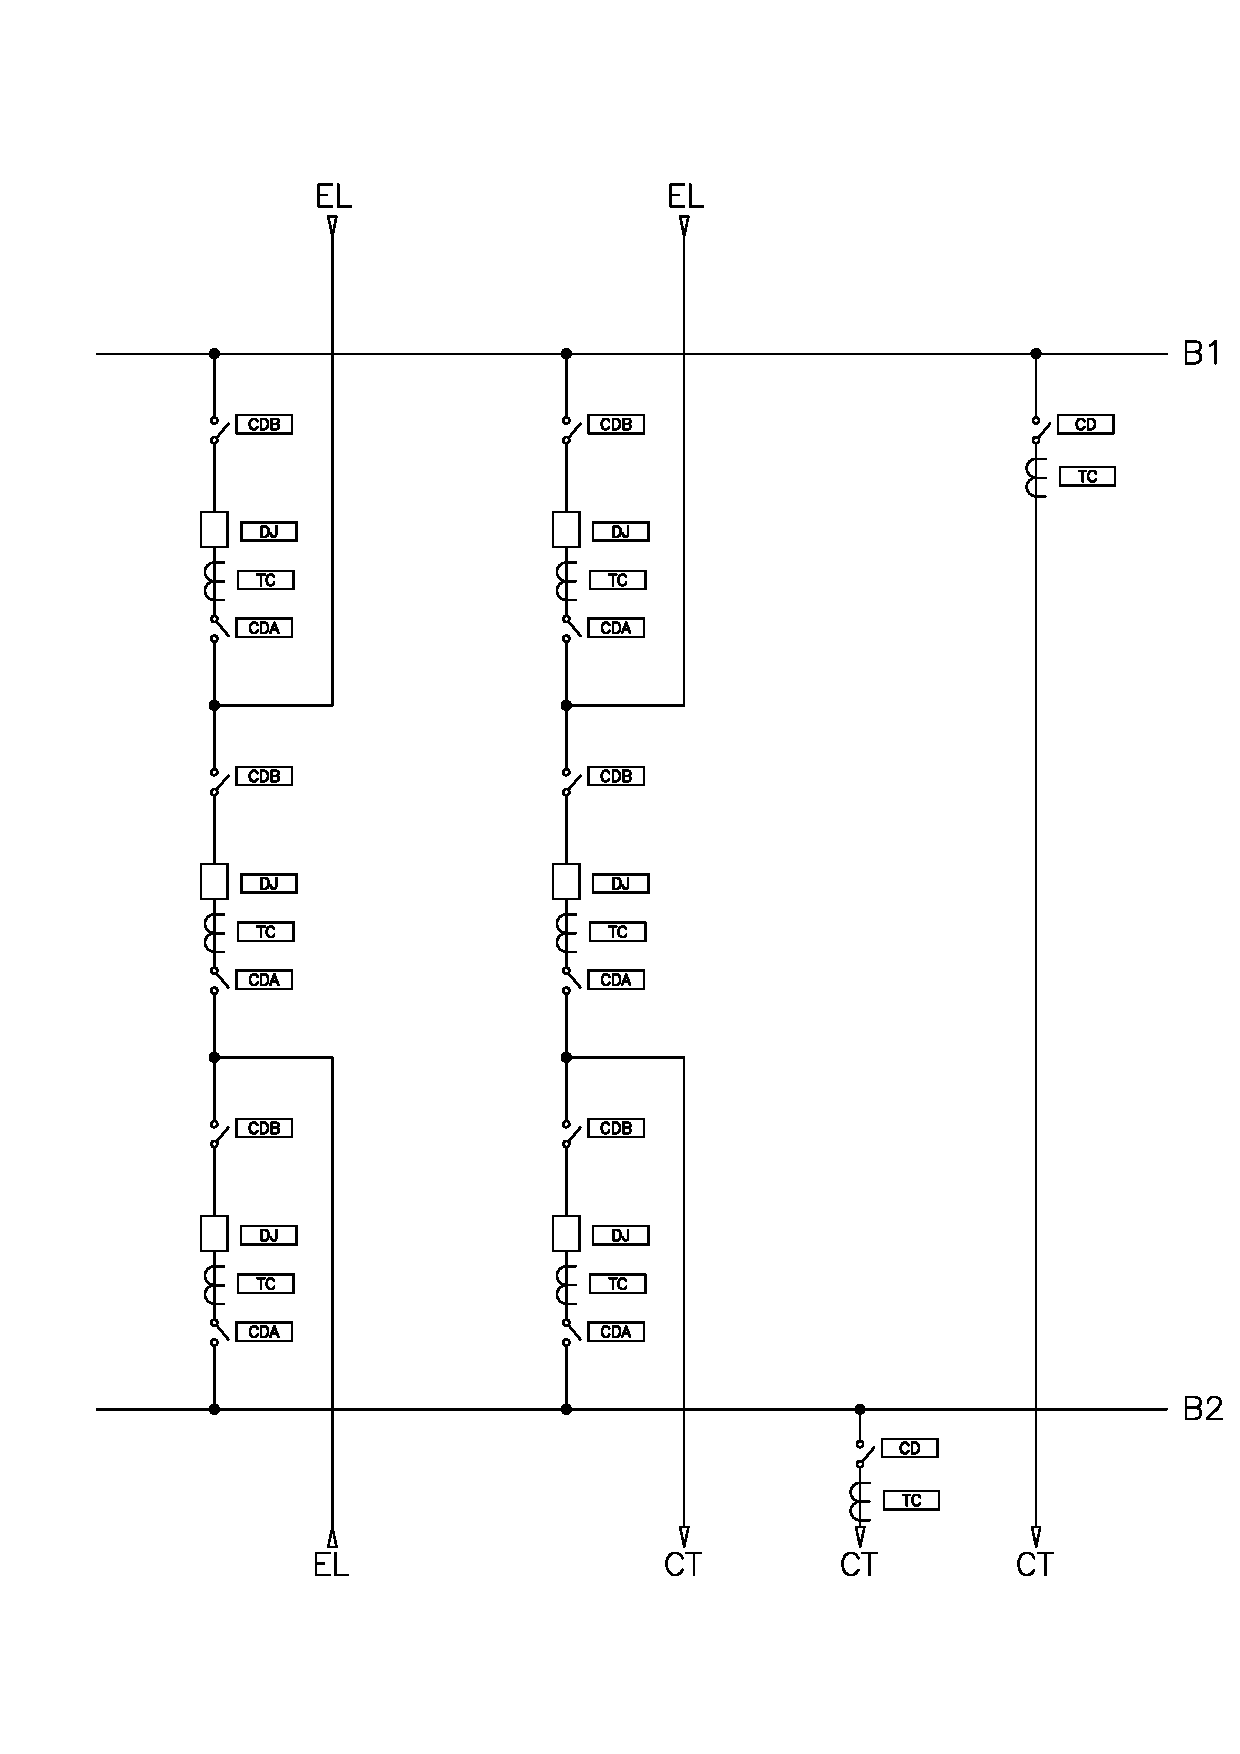
\includegraphics[width=10.8cm]{11BD-D1-2M.pdf}
				\legend{Fonte: Do autor}
				\label{fig:BD-D1/2M}
				\end{figure}
%		\subsection{Barra Dupla com Disjuntor e Um Terço (BD-D1/3)}
		\subsection{Barra Dupla com Disjuntor Duplo (BD-Dd)}
			Para subestações muito específicas, com reduzido número de \textit{bays} e alta capacidade de potência por \textit{bay}, como por exemplo, em conexões de usinas nucleares, a configuração em barra dupla com disjuntor duplo pode ser uma solução apropriada. A \autoref{fig:BD-DD} ilustra a situação. É importante observar que nesta configuração não há disjuntor de interligação de barras. Embora esta configuração seja de alto desempenho, uma eventual perda das duas barras (baixa probabilidade) provoca a perda total de conectividade na subestação, ficando, sob este aspecto, em desvantagem em relação às configurações em barra dupla com disjuntor e meio e barra dupla com disjuntor e um terço. Um pátio com esta configuração de barra é de custo elevado e só deve ser aplicado quando um estudo quantitativo criterioso embasar a decisão.\par
			\begin{figure}[!htb]
				\caption{Configuração Barra Dupla com Disjuntor Duplo}
				\centering
				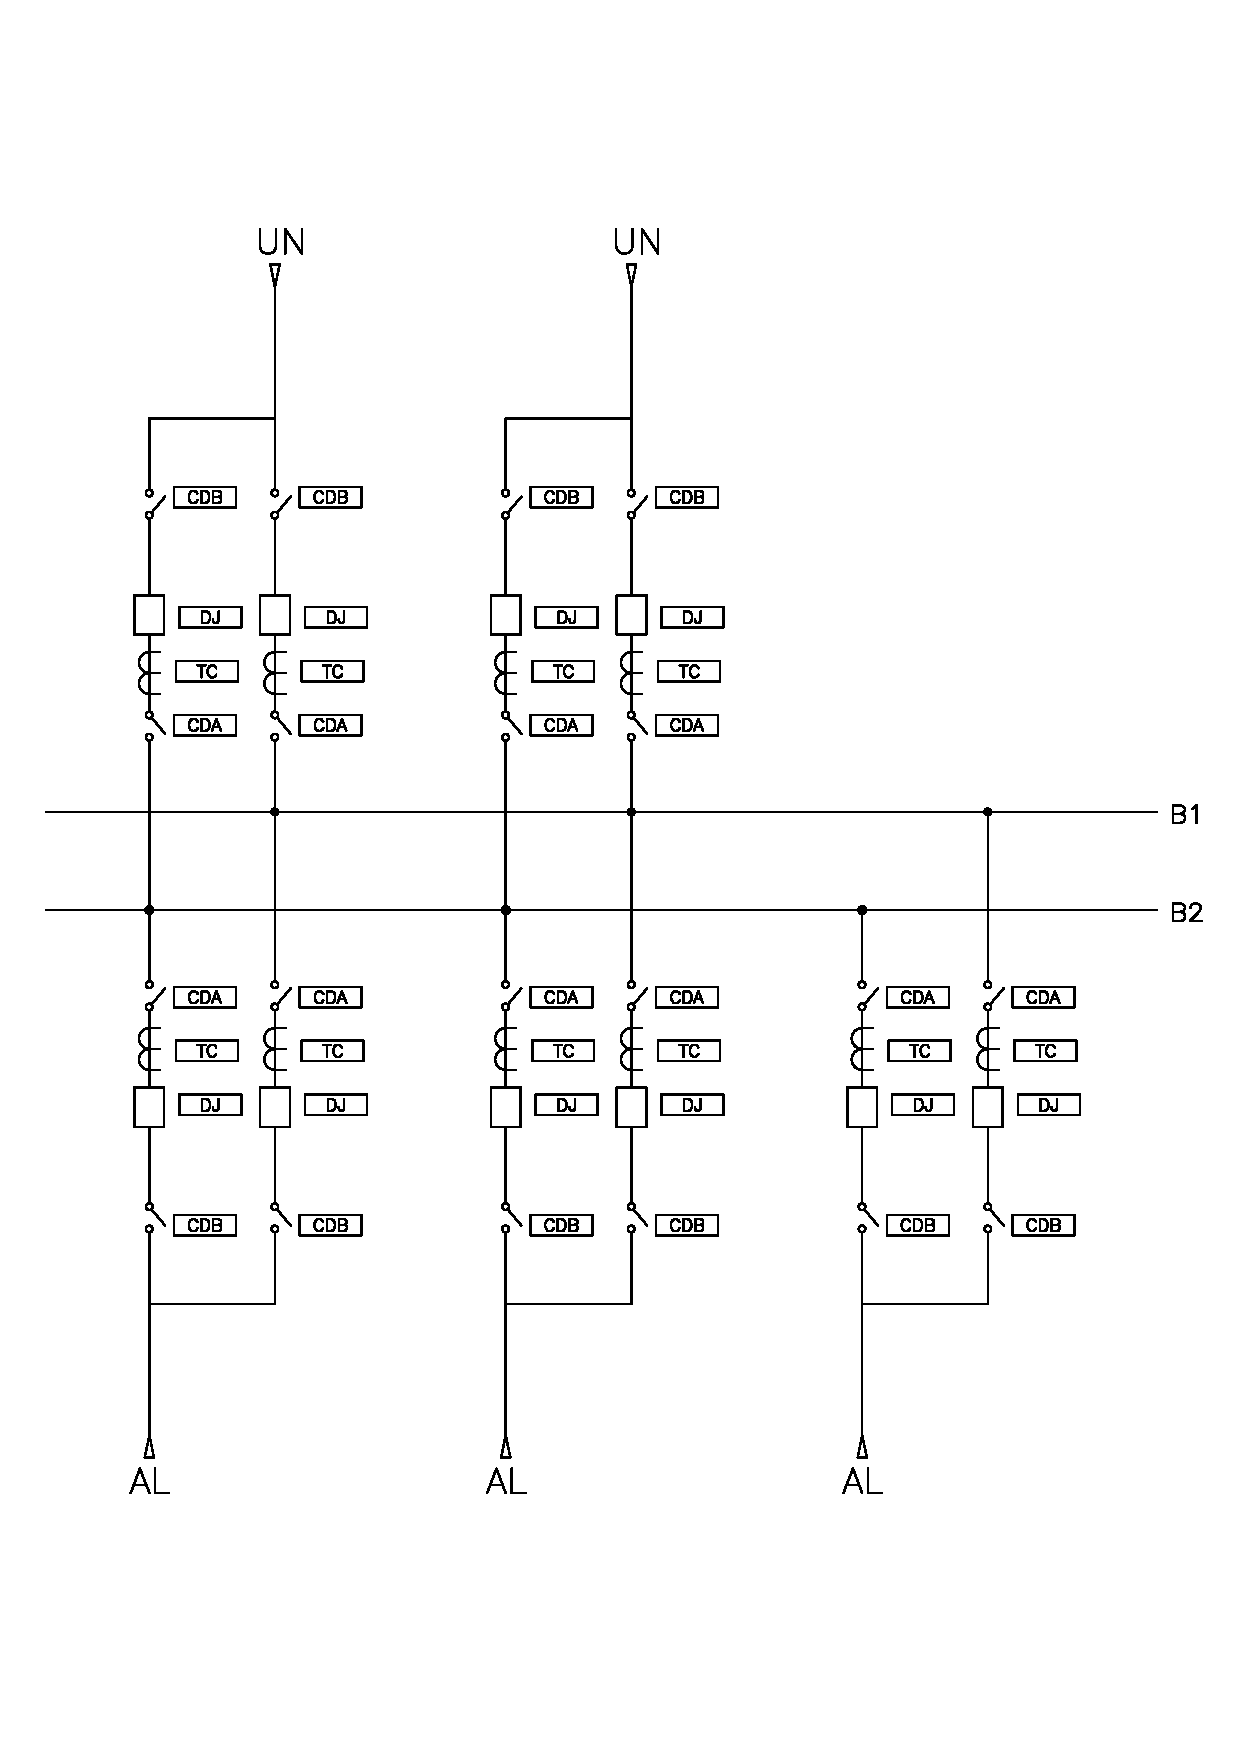
\includegraphics[width=10.8cm]{13BD-DD.pdf}
				\legend{Fonte: Do autor}
				\label{fig:BD-DD}
				\end{figure}

% ---------------------------------------------------
% Capítulo 3
% ---------------------------------------------------

\chapter{Problemática da Demanda de Carga da Subestação Camboriú (CBU) -- SC}
\label{chap:demCarga}
\textcolor{red}{\lipsum}
% ---------------------------------------------------
% Capítulo 4
% ---------------------------------------------------

\chapter{Solução de Ampliação para a Subestação Camboriú}
\label{chap:solAmp}
\textcolor{red}{\lipsum}
% ---------------------------------------------------
% Capítulo 5
% ---------------------------------------------------

\chapter{Como é feito em outras partes do mundo}
\label{chap:asbuiltAbroad}
\textcolor{red}{\lipsum}

% ---------------------------------------------------
% Conclusão
% ---------------------------------------------------
\chapter*[Conclusão]{Conclusão}
\textcolor{red}{\lipsum}

\bibliography{refs}